% \documentclass[acmtocl,acmnow,hyperref]{acmtrans2m}
\documentclass[11pt]{article}
\usepackage{verbatimfiles}
\usepackage{amssymb}
\usepackage{amsmath}
\usepackage{url}
\usepackage[pdftex,usenames]{color}
\usepackage[pdftex]{graphicx}  
\DeclareGraphicsExtensions{.pdf}  
\usepackage[pdftex,bookmarks=true,bookmarksnumbered=true,hypertexnames=false,breaklinks=true]{hyperref}
\hypersetup{
  pdfauthor = {Jean Utke},
  pdftitle = {OpenAD: A tool for automatic differentiation of Fortran codes},
  pdfsubject = {TOMS article},
  pdfkeywords = {OpenAD,automatic differentiation, algorithms},
  pdfcreator = {LaTeX with hyperref package},
  pdfproducer = {dvips + ps2pdf}sh	
}
\pdfadjustspacing=1

% make paragraphs show up in the bookmarks
\setcounter{secnumdepth}{6}
\setcounter{tocdepth}{6}

\fboxsep.5mm

% names and CS terms
\newcommand{\angel}{angel}
\newcommand{\entry}{entry}
\newcommand{\exit}{exit}
\newcommand{\Loop}{loop}
\newcommand{\EndLoop}{endloop}
\newcommand{\branch}{branch}
\newcommand{\EndBranch}{endbranch}
\newcommand{\basicblock}{basicblock}
\newcommand{\mfefninety}{mfef90}
\newcommand{\OpenADF}{OpenAD/F}
\newcommand{\OpenAD}{OpenAD}
\newcommand{\OpenADFortTk}{OpenADFortTk}
\newcommand{\OpenAnalysis}{OpenAnalysis}
\newcommand{\OpenSixtyFour}{Open64}
\newcommand{\saxpy}{saxpy}
\newcommand{\xaif}{XAIF}
\newcommand{\xaifBooster}{xaifBooster}
\newcommand{\whirl}{whirl}
\newcommand{\whirlToxaif}{whirl2xaif}
\newcommand{\whirlTof}{whirl2f}
\newcommand{\xaifTowhirl}{xaif2whirl}

% math
\newcommand{\R}{I\!\!R}
\newcommand{\bmC}{\mbox{\bf\em C}}
\newcommand{\bmf}{\mbox{\bf\em f}}
\newcommand{\bmfp}{\mbox{\bf\em f$\,^\prime\!\!$}}
\newcommand{\bmg}{\mbox{\bf\em g}}
\newcommand{\bmI}{\mbox{\bf\em I}}
\newcommand{\bmJ}{\mbox{\bf\em J}}
\newcommand{\bmu}{\mbox{\bf\em u}}
\newcommand{\bmv}{\mbox{\bf\em v}}
\newcommand{\bmw}{\mbox{\bf\em w}}
\newcommand{\bmx}{\mbox{\bf\em x}}
\newcommand{\bmy}{\mbox{\bf\em y}}

% environments
\newcommand{\code}[1]{{\small\tt{#1}}}
\newcommand{\refcan}[1]{(C\ref{#1})}
\newcommand{\refsec}[1]{{Sec.~\ref{#1}}} 
\newcommand{\refsecBS}[1]{{Section~\ref{#1}}} 
\newcommand{\reffig}[1]{{Fig.~\ref{#1}}} 
\newcommand{\reffigBS}[1]{{Figure\ref{#1}}} 
\newcommand{\reftab}[1]{{Table~\ref{#1}}} 
\newcommand{\refalg}[1]{{Alg.~\ref{#1}}} 
\newcommand{\refalgBS}[1]{{Algorithm~{#1}}} 
\newcommand{\refeqn}[1]{{(\ref{#1})}} 
\newcommand{\refdef}[1]{{Def.~(\ref{#1})}} 
\newtheorem{Can}{Canonicalization}

% \markboth{Lots Of Authors et al.}{OpenAD}

\begin{document}

% \title{OpenAD/F: A tool for automatic differentiation of Fortran codes}


% \author{PATRICK HEIMBACH, CHRIS HILL, DERYA OZYURT, CARL WUNSCH\\Massachusetts Institute of Technology\\
%   MIKE FAGAN, NATHAN TALLENT \\Rice University\\
%   MICHELLE STROUT, JEAN UTKE \\Argonne National Laboratory 
%   \and
%   UWE NAUMANN\\Rheinisch Westf\"alische Techinische Hochschule Aachen}

\begin{center}
  {\Large OpenAD/F: A tool for automatic differentiation \\ of Fortran codes}\\[1ex]
  {\tiny
    PATRICK HEIMBACH, CHRIS HILL, DERYA OZYURT, CARL WUNSCH\\Massachusetts Institute of Technology\\
    MIKE FAGAN, NATHAN TALLENT \\Rice University\\
    MICHELLE STROUT, JEAN UTKE \\Argonne National Laboratory \\
    UWE NAUMANN\\Rheinisch Westf\"alische Techinische Hochschule Aachen}
\end{center}

\begin{abstract}

  The \OpenADF\ tool allows the evaluation of first and second order
  derivatives of functions defined by a program written in Fortran90/77.

  {\color{red} JU: Ehmm - qualify the above } 

  The derivative evaluation is performed by Fortran 90 code resulting
  from the analysis and transformation of the original program that
  defines the function of interest.  The code transformation follows the
  basic principles of automatic differentiation.  In difference to most
  other automatic differentiation tools \OpenADF\ uses components 
  provided by the \OpenAD\ framework which supports a relatively 
  easy extension of the code transformations
  in a language indepdendent fashion. 
  It uses code analysis results
  implemented in the \OpenAnalysis\ component.  The interface to the
  language independent transformation engine is an xml abstract
  interface format, called \xaif\ that is specified through an xml
  schema.  The implemented transformation algorithms allow efficient
  derivative computations utilizing locally optimized cross country
  sequences of vertex, edge and face elimination steps.  Specifically,
  for the generation of adjoint codes, \OpenADF\ supports various code
  reversal schemes with hierachical checkpointing at the subroutine
  level.  The Fortran specific front and back end to this transformation
  engine is based on the \OpenSixtyFour\ compiler.
\end{abstract}


% \category{G.1.4}{Quadrature and Numerical Differentiation}{Automatic differentiation}
% \category{D.3.4}{Processors}{Code generation, Compilers}
% \category{F.3.2}{Semantics of Programming Languages}{Program analysis}
% \category{G.1.6}{Optimization}{Gradient methods}

% \terms{Algorithms, Performance}

% \keywords{Automatic differentiation,  source transformation, adjoint compiler}



% \begin{bottomstuff} 
%   P.~Heimbach, C.~Hill, D.~Ozyurt, and C.~Wunsch, Massachusetts Institute of Technology, 
%   Boston, MA 02139;\newline
%   M.~Fagan, N.~Tallent, Rice University, 
%   Houston, TX 77251;\newline
%   M.~Strout, J.~Utke, Argonne National Laboratory, 
%   Argonne, IL 60439;\newline
%   U.~Naumann, Rheinisch Westf\"alische Techinische Hochschule Aachen, 
%   D-52056 Aachen, Germany;\newline
%   Funding for the ACTS project is provided by NSF under ITR contract OCE-0205590
%   for a three year period that started in September 2002.
% \end{bottomstuff}
% \maketitle

% #########################################################################################
\section{Introduction} \label{sec:Introduction}

The basic principles of automatic differentiation (AD), see also \refsec{sec:ADIntro}, 
have been known for several decades \cite{wengert}
but only during the last 15 years have the tools implementing AD found a significant use in 
optimization, data assimilation, and other applications in need of efficient and accurate 
derivative information. 
As a consequence of the wider use of AD, 
a variety of tools have been developed that address specific 
application requirements or programming languages. 
The  AD community's website \cite{autodiffWeb} 
provides a comprehensive overview of the tools that 
are currently available. 
One can categorize two user groups of AD tools. 
On one side are the casual users 
with small-scale problems applying AD mostly in a black-box fashion 
and demanding minimal user intervention. 
This category also includes the use of AD tools in  computational 
frameworks such as NEOS \cite{neosWeb}.
On the other side are experienced AD users aiming for highly efficient 
derivative computations.
Their need for efficiency is dictated by the 
computational complexity of models that easily reaches the limits of  current 
supercomputers. 
With the emphasis on efficiency some sacrifices on the support of 
language features are acceptable for this user group.  

\subsection{Motivation}
One of the most demanding applications of AD is the computation of gradients for 
data assimilation on large scale models used in oceanography and climate research. 
These applications clearly fall in the category of advanced uses.
An evaluation of the available tools revealed some shortcomings from the perspectives 
of the tool users as well as the tool developers. 

From  the AD tool  {\em users point of view} there is a need for a substantial 
flexibility of the AD tools. 
We pointed out that the most demanding  numerical models 
operate on the limit of the computing capacity of state of the art facilities. 
Usually the model code itself is specifically adapted to fit certain 
hardware characteristics. 
Consequently the AD tools code generation should be adapted in the same fashion. 
Some of these specific solutions may be folded into the generic code transformation engine 
but in many situation this is not appropriate.
Consequently the AD tool should offer flexibility at various levels of the 
transformation from simple textual preprocessing of the code down to the 
changes the to the generice code transformation engine.
This is the user rationale for developing an open source tool where {\em all} 
components may be modified by to suit specific 
needs.  
A modular tool design with clearly defined interfaces supports such 
user interventions. 
As this design instigates a staged 
transformation, see \refsec{ssec:manualPipeline}, 
each transformation stage presents a opportunity to check and modify the 
results. 

From the AD tool {\em developers point of view} it is very apparent that 
many AD tools share the same basic algorithms while on the other hand 
there is a relatively steep hurdle to establish a working environment 
for the source to source transformation. 
This is true for a parsing front-end that turns the textual program into a 
compiler-like internal representation, an environment that allows the 
transformations  of this internal representation and finally the unparser that 
returns the transformed internal representation back into a textual format of the 
original programming language. An modular, open-source tool that faciliates 
the integration of new transformation into an existing environment 
allows for a much quicker implementation of new or modified  transformations.
Finally, a modular design permits the reuse of the same transformation algorithms 
for multiple target languages as long as there are parsing front-ends adhering to the 
same internal representation.

These issues became the motivation for the 
Adjoint Compiler Technology \& Standards (ACTS) project \cite{actsWeb}.
This project is a collaborative
research and development effort of MIT, Argonne National Laboratory, 
Univeristy of Chicago, and Rice University. 
It focusses on  next-generation tool development and 
application of AD to problems in oceanography and chemical engineering.
The main result of this effort is an infrastructure for the language independent 
development and use of AD algorithms. 

\subsection{Overview}
\OpenADF \cite{openadWeb}
is the Fortran incarnation of the AD framework \OpenAD.
The C/C++ oriented tool ADIC v2.0 \cite{adicWeb}
is based on the same framework but is 
not subject of this article.
\begin{figure}
  \centering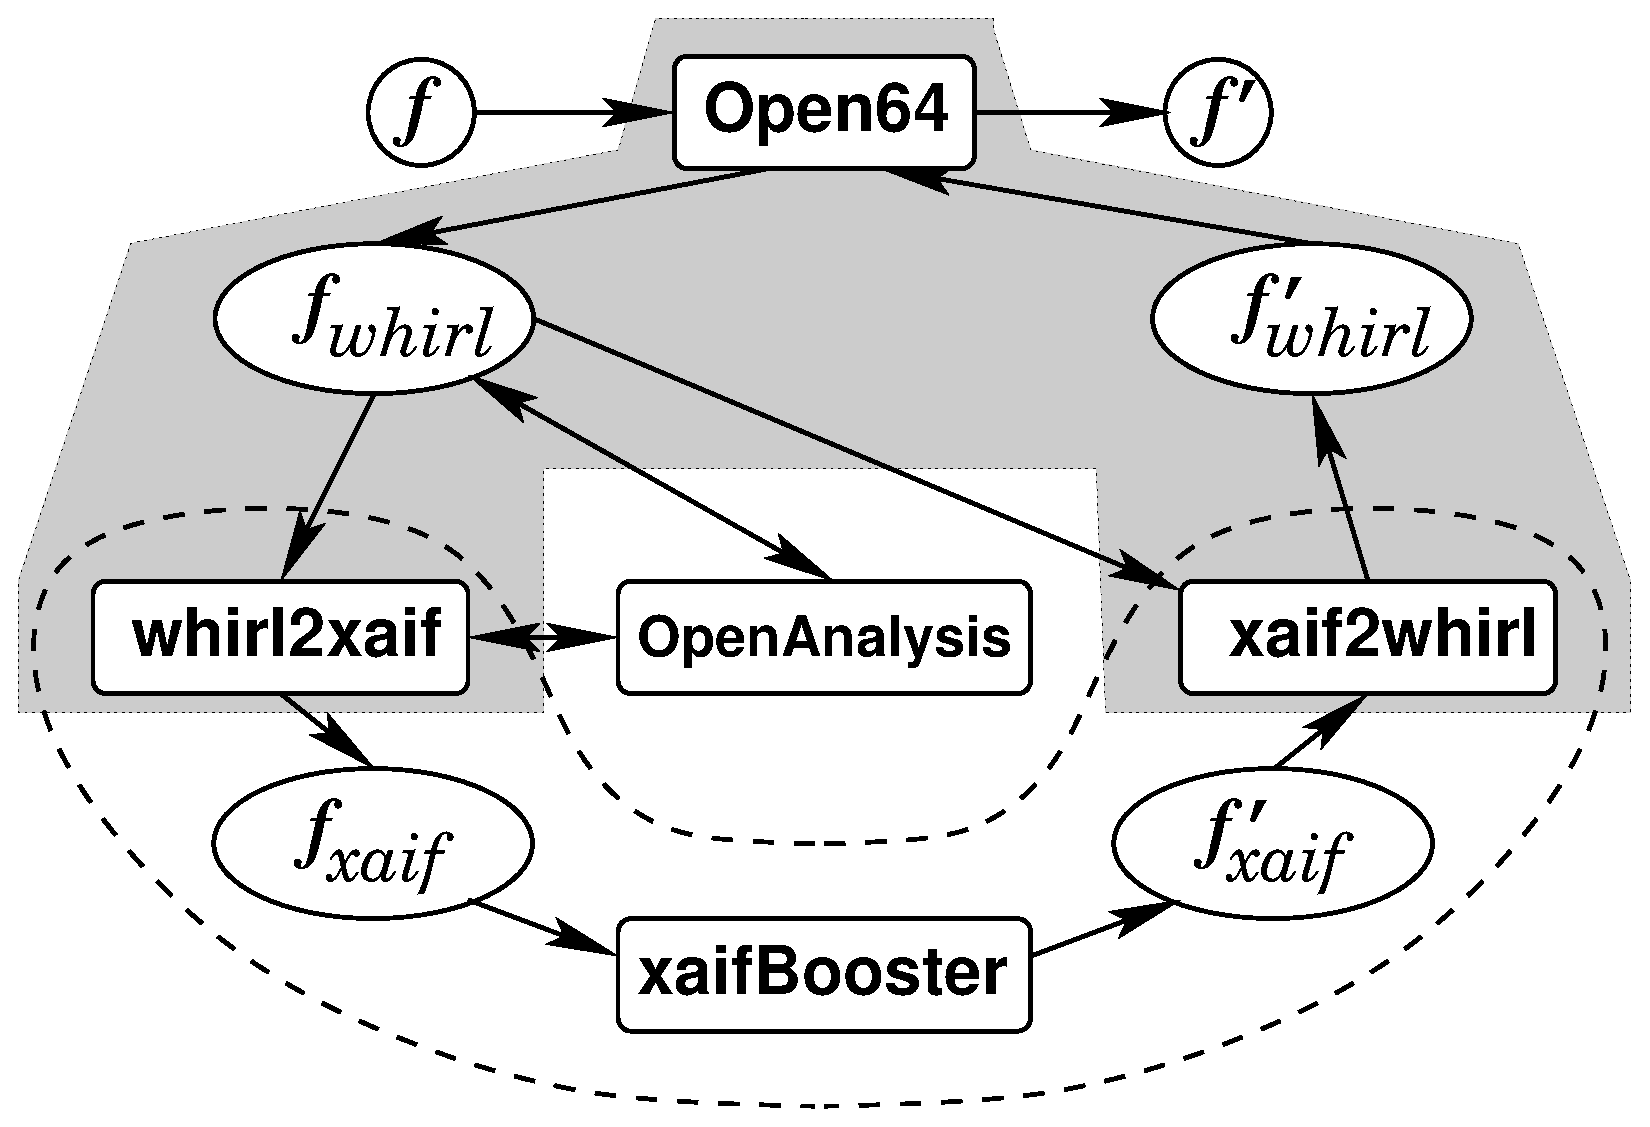
\includegraphics[width=.5\textwidth]{overview}
  \caption{\OpenADF\ components and pipeline} \label{fig:overview}
\end{figure}
\OpenADF\ has  a modular design. 
The collaboration  of the \OpenADF\ components is illustrated in 
\reffig{fig:overview}.
Our input is some numerical model given as a Fortran program 
$\bmf$.
The \OpenSixtyFour\cite{open64Web}
front-end performs a lexical, 
syntactic, and semantic analysis and produces an 
intermediate representation of $\bmf$, here denoted by $\bmf_{\whirl}$, 
in the so-called \whirl\ format.
\OpenAnalysis\ is used to build call and control flow graphs and  perform 
code analyses such as alias, activity, side-effect analysis.
This information is used by 
\whirlToxaif\ to construct a representation of the numerical core of $\bmf$ in
\xaif\ format shown as $\bmf_{xaif}$.  
A differentiated version of $\bmf_{xaif}$ is derived by an 
algorithm that is implented in \xaifBooster\ and is again respresented 
\xaif\ as $\bmfp_{xaif}$.
The information in $\bmfp_{xaif}$ and the original $\bmf_{\whirl}$ are used by 
\xaifTowhirl\ to construct a 
\whirl\ representation $\bmfp_{\whirl}$ of the differentiated code. 
The unparser of 
\OpenSixtyFour\ transforms $\bmfp_{\whirl}$ into Fortran90, thus completing
the semantic transformation of a program $\bmf$ into
a differentiated program $\bmfp$.
The gray shaded area encloses the language specific front-end that can potentially
be replaced by front-ends for languages other than Fortran. 
For instance, the new version of ADIC \cite{HoNo01} couples a C/C++ 
front-end 
based on the EDG parser \cite{edgWeb} and uses ROSE in combination with SAGE~3 \cite{roseWeb} 
as internal representation in combination with language independent components of \OpenAD.

In \refsec{sec:ADIntro} we discuss the basic concepts of AD as relevant for 
the description of \OpenAD, \refsec{sec:openadcomponents} discusses the components 
that make up \OpenADF, and \refsec{sec:Usage} details the usage of the tool. 
Two applications further illustrate the tool usage in \refsec{sec:application} and 
we conclude with a section on future devlepments.

% #########################################################################################
\section{AD Concepts}\label{sec:ADIntro}

In this section we present the terminology and basic concepts that 
we will refer to throughout this paper. 
A detailed introduction to AD can be found in \cite{Gri00}.
The interested reader should also consider the proceedings of AD 
conferences \cite{CG91,BBCG96,CFG+01,BCH+05}.

We present the concepts and resulting transformations 
with respect to the input source code 
in a bottom up fashion.  
We first consider elemental numerical operations, 
then their control flow context within a subroutine and finally the entire program 
consisting of several subroutines in a call graph. 

We view a given numerical model as a 
vector valued function $\bmy=\bmf(\bmx): \R^n\mapsto \R^m$ that is implemented 
as a computer program in a language such as Fortran, C, or C++. 

% -----------------------------------------------------------------------------------------
\subsection{Computational Graphs} \label{ssec:computationalGraphs}

Without loss of generality we can simply assume that an evaluation of $\bmf(\bmx)$ for  
a specific value of $\bmx$ can be represented by a sequence of 
elemental operations $v_j=\phi_j(\ldots,v_i,\ldots)$. 
The $v_i$ represent the vertices $\in V$ in the correspong corresponding computational 
graph $G=(V,E)$. The edges $(i,j)\in E$ in this graph are the direct dependencies 
$v_i\prec v_j$ implied by the elemental $v_j=\phi_j(\ldots,v_i,\ldots)$.
The elemental operations $\phi$ are differentiable on open subdomains. 
Each edge $(i,j)\in E$ has an attached local partial derivative 
$c_{ji}=\frac{\partial v_j}{\partial v_i}$. 
The central principle of AD is 
the application of the chain rule to the elemental $\phi$, that is 
multiplications and additions of the  $c_{ji}$.  

Like most of the AD literature we follow a specific numbering scheme for the vertices $v_i$.
We presume $q$ intermediate values
$v_j = \phi_j(\ldots,v_i,\ldots), v_j\in Z$
for $j=1,\ldots,q+m$ and $h,i=1-n,\ldots,q,$ $j>h,i$. 
The $n$ {\em independent}
variables $x_1,\ldots,x_n$ correspond to 
$v_{1-n},\ldots,v_0, v_i\in X$. 
We consider the 
computation of derivatives of the {\em dependent} variables 
$y_1,\ldots,y_m$ represented by $m$ variables $v_{q+1},\ldots,v_{q+m}, v_j\in Y$
with respect to the independents. 
The depdendency $v_i<v_j$ implies $i<j$. 
The {\em forward mode} of AD propagates directional derivatives
as 
\begin{equation} \label{eqn:fm}
  \dot{v}_j= \sum\limits_i\frac{\partial \phi_j}{\partial v_i}\dot{v}_i 
  \quad \text{for}~~j=1,\ldots,q+m.
\end{equation} 
In {\em reverse mode} we compute adjoints of the arguments of the $\phi_j$
as a function of local partial derivatives and the 
adjoint of the variable on the left-hand side
\begin{equation} \label{eqn:rm}
  \overline{v}_i= \sum\limits_j\frac{\partial \phi_j}{\partial v_i}\overline{v}_j 
  \quad \text{for}~~j=1,\ldots,q+m.
\end{equation} 
In practice, the sum in \refeqn{eqn:rm} is often split into individual increments 
associated with each statement in which $v_i$ occurs as an argument 
$\overline{v}_i=\overline{v}_i+\overline{v}_j * \frac{\partial \phi_j}{\partial v_i}$.

Equations \refeqn{eqn:fm} and \refeqn{eqn:rm} can be used to accumulate 
the (local) Jacobian $\bmJ(G)$
of $G$, see also \refsec{ssec:elimMeth}. 
% Obviously \refeqn{eqn:rm}  indicates that the dependencies of $\overline{v}_j$ and 
% $\overline{v}_i$ are reversed to those of $v_j$ and $v_i$. At the same time \refeqn{eqn:rm}
% requires all the values of the $\frac{\partial \phi_j}{\partial v_i}$ in reverse order. To make them 
% available we store them in a stack. In the  AD literature this is commonly called the {\em tape}. 

In a source transformation context we want to generate code for all $\bmf(\bmx)$
in the domain and because the above construction disregards control flow it is 
impractical here. Instead we simply consider the statements contained in a 
\basicblock\  as a section of code below the granularity of control flow and 
construct our computational (sub) graph for a \basicblock.   

% -----------------------------------------------------------------------------------------
\subsection{Elimination Methods} \label{ssec:elimMeth}
Let $\bmf$ represent a single \basicblock\ that is subject to preaccumulation.
For notational simplicity and without loss of generality we assume that the 
dependent variables are mutually independent. 
This situation can always be
reached by introducing auxiliary assignments.
Consider the small example in \reffig{fig:toyBB}.
\begin{figure}[h]
  \begin{center}
    \begin{minipage}{.4\textwidth}
      \verbatimfile{code/straightLine.f90}
    \end{minipage}
  \end{center}
  \caption{Example of code contained in a \basicblock}\label{fig:toyBB}
\end{figure}
Reformulating the example in terms of 
results of elemental operations $\phi$ assigned to unique intermediate 
variables $v$ we have 
\begin{equation}\label{eqn:sampleCode}
  \begin{split}
    v_1&=v_{-1}+v_0;~v_2=\sin(v_0);~v_3=v_1+v_2;~v_4=v_1*v_3; \\
    v_5&=\sqrt{v_3};~v_6=\cos(v_4);~v_7=-v_5 \quad .\\
  \end{split}
\end{equation}
In the tool this modified representation is created as part of the linearization transformation, see 
\refsec{sssec:linearization}.
In \reffig{fig:elims}~(a) we show the computational graph $G$ for this representation.
\begin{figure}
  \centering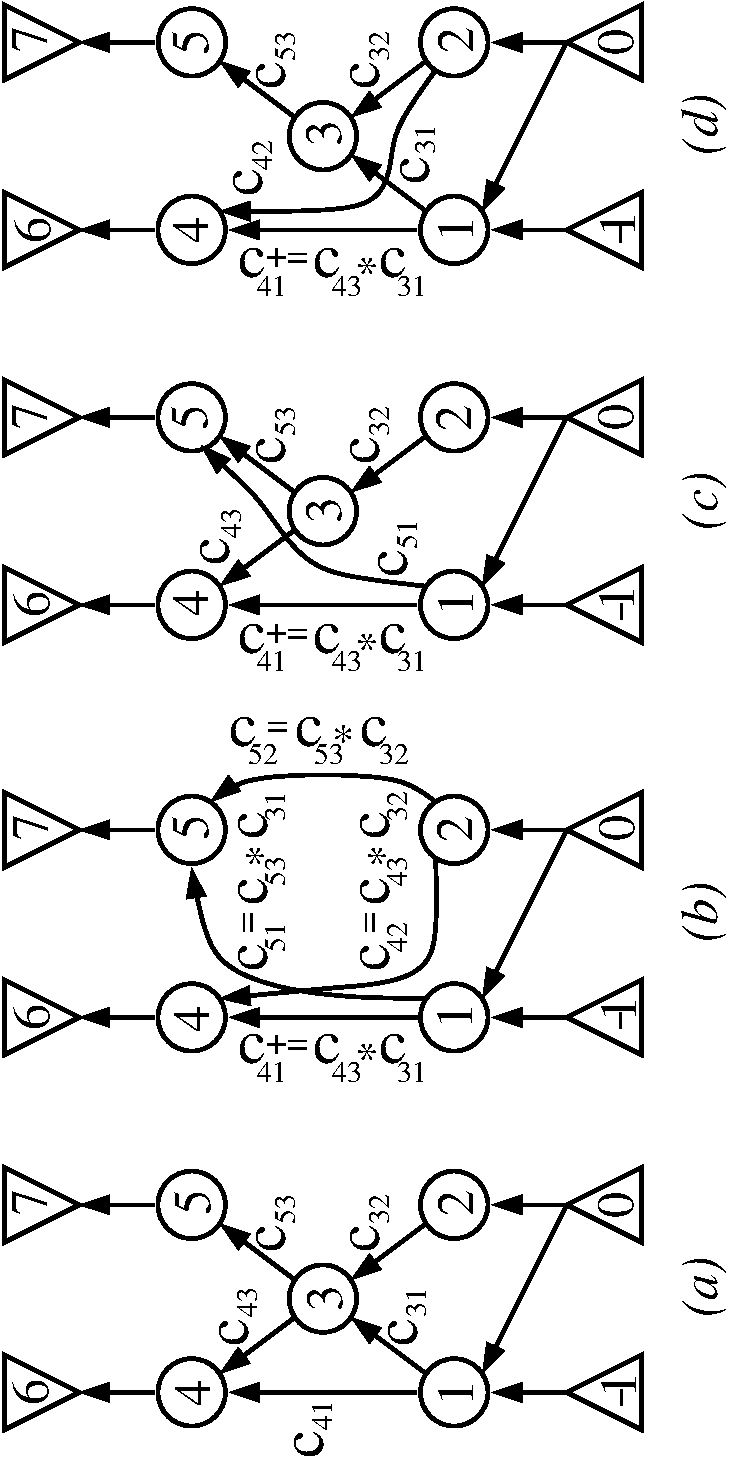
\includegraphics[width=.7\textwidth]{elims}
  \caption{
    (a) Computational graph $G$ for \refeqn{eqn:sampleCode}, 
    (b) eliminate vertex 3 from $G$, 
    (c) front eliminate edge $(1,3)$ from $G$, 
    (d) back eliminate edge $(3,4)$ from $G$} 
  \label{fig:elims}
\end{figure}
The edges $(i,j)\in E$ are labeled with partial derivatives
$c_{ji}$, for instance, in the 
example we have $c_{64}=-\sin(v_4)$.
In the tool, this graph is generated as part of the algorithm described in 
\refsec{sssec:BBPreacc}.
Jacobian preaccumulation can be interpreted as eliminations in $G$.
The graph-based elimination steps are categorized in vertex, edge, and face 
eliminations. 
In $G$ a vertex $j \in V$ is eliminated by connecting its predecessors with
its successors \cite{GrRe91}.
An edge $(i,k)$ with
$i \prec j$ and $j \prec k$ is labeled with
$c_{ki}+c_{kj} \cdot c_{ji}$ if it existed before the elimination of $j.$
We say that {\em absorption} takes place.
Otherwise, $(i,k)$ is generated as {\em fill-in} and labeled
with $c_{kj} \cdot c_{ji}$
The vertex $j$ is removed from
$G$ together with all incident edges. 
\reffig{fig:elims}~(b) shows the result of eliminating vertex $3$
from the graph in \reffig{fig:elims}~(a).

An edge $(i,j)$ is {\em front eliminated} by connecting $i$ with all successors
of $j$, followed by removing $(i,j)$ \cite{Nau00a}.
The corresponding structural modifications of the c-graph in
\reffig{fig:elims}~(a) are shown in
\reffig{fig:elims}~(c) for front elimination of $(1,3).$
The new edge labels are given as well.
Edge-front elimination eventually leads to intermediate vertices in $G$
becoming
{\em isolated}; that is, these vertices no longer have predecessors.
Isolated vertices are simply removed from $G$ together
with all incident edges.

Back elimination of an edge
$(i,j) \in E$ results in connecting all predecessors of $i$
with $j$ \cite{Nau00a}.
The edge $(i,j)$ itself is removed from $G.$
The back elimination of $(3,4)$ from the graph in \reffig{fig:elims}~(a) 
is illustrated in \reffig{fig:elims}~(d). 
Again, vertices can become isolated as a result of edge-back elimination
because they no longer have successors.
Such vertices are removed from $G.$

Numerically the elimination is the application of 
the chain rule, that is, a sequence of {\em fused-multiply-add} (fma) operations
\begin{equation}\label{eqn:fma}
  c_{ki}=c_{ji}*c_{kj}\hspace*{1ex}(+c_{ki}) 
\end{equation}
where the additions in parenthesis take place only  in the case of 
absorption or otherwise fill-in is created 
as described above.

Aside from special cases a single vertex or edge elimination will result in more
than one fma. {\em Face elimination} was introduced 
as the elimination operation with the finest granularity of exactly 
one multiplication\footnote{Additions are not necessarily directly coupled.} 
per elimination step.

Vertex and edge elimination steps have an 
interpretation in terms of vertices and edges
of $G$, whereas face elimination is performed on 
the corresponding directed line graph $\cal G.$
Following \cite{ElimTechMP}, we define the directed line graph $\cal G=(V,E)$ 
corresponding to $G=(V,E)$ as follows:
\[
{\cal V}=
\left\{\,\framebox{$i,j$}      :(i,j)\in E \right\} \cup 
\left\{\,\framebox{$\oplus,j$} :v_j  \in X \right\} \cup 
\left\{\,\framebox{$i,\ominus$}:v_i  \in Y \right\}
\] 
and 
\begin{align*}
  {\cal E}
  &=    \left\{\big(\;\framebox{$i,j$}     \,,\framebox{$j,k$}      \;\big): (i,j),(j,k) \in E        \right\} \\
  &\cup \left\{\big(\;\framebox{$\oplus,j$}\,,\framebox{$j,k$}      \;\big): v_j\in X \land (j,k)\in E\right\} \\
  &\cup \left\{\big(\;\framebox{$i,j$}     \,,\framebox{$j,\ominus$}\;\big): v_j\in Y \land (i,j)\in E\right\} 
  \quad . \\
\end{align*}
That is, 
we add a source vertex $\oplus$ and a sink vertex 
$\ominus$ to $G$ connecting all independents to $\oplus$
and all dependents to $\ominus$. $\cal G$ has   
a vertex $ v \in \cal V$ for each edge in the extended $G$, 
and $\cal G$ has an edge $ e \in \cal E$ for each 
pair of adjacent edges in $G$. \reffig{fig:face_elims} gives an 
example of constructing the directed line graph in (b) from the graph in (a) 
which is the graph from \reffig{fig:elims}(a) extended by the source and sink vertex.   
All intermediate vertices $\framebox{$i,j$} \in \cal V$ inherit the labels  
$c_{ji}$. In order to formalize face elimination, it is advantageous to move away
from the double-index notation and use one that is based on a topological
enumeration of the edges in $G.$ Hence, ${\cal G}=({\cal V}, {\cal E})$ 
becomes a DAG with ${\cal V} \subset I\!\!N$ and
${\cal E} \subset I\!\!N \times I\!\!N$ and
certain special properties.
The set of all predecessors of $j \in {\cal V}$ is denoted as $P_j.$ 
Similarly, $S_j$ denotes the set of its successors in $\cal G.$ 
A vertex 
$j \in \cal V$ is called {\em isolated} if either 
$P_j=\emptyset$ or
$S_j=\emptyset.$ 
Face elimination is defined in \cite{ElimTechMP}
between two incident intermediate vertices $i$ and $j$ in $\cal G$ as follows:
\begin{enumerate}
\item If there exists a vertex $k \in \cal V$ such that $P_k = P_i$ and
  $S_k = S_j,$ then
  set $c_k = c_k + c_j c_i$ {\em (absorption)};
  else ${\cal V}={\cal V} \cup \{k'\}$ with a new vertex $k'$ such that
  $P_{k'} = P_i$ and $S_{k'} = S_j$
  {\em (fill-in)} and labeled with $c_{k'} = c_j c_i.$
\item Remove $(i,j)$ from $\cal E.$
\item Remove $i \in \cal V$ if it is isolated. Otherwise, if there exists a vertex $i' \in \cal V$ such that
  $P_{i'} = P_i$ and $S_{i'} = S_i,$ then
  \begin{itemize}
  \item set $c_i=c_i + c_{i'}$ {\em (merge)};
  \item remove $i'.$
  \end{itemize}
\item Repeat Step 3 for $j \in \cal V.$
\end{enumerate}
In \reffig{fig:face_elims}~(c) we show the elimination of $(i,j) \in \cal E$,
where $i=\framebox{$1,3$}$ and $j=\framebox{$3,4$}$.

\begin{figure}
  \centering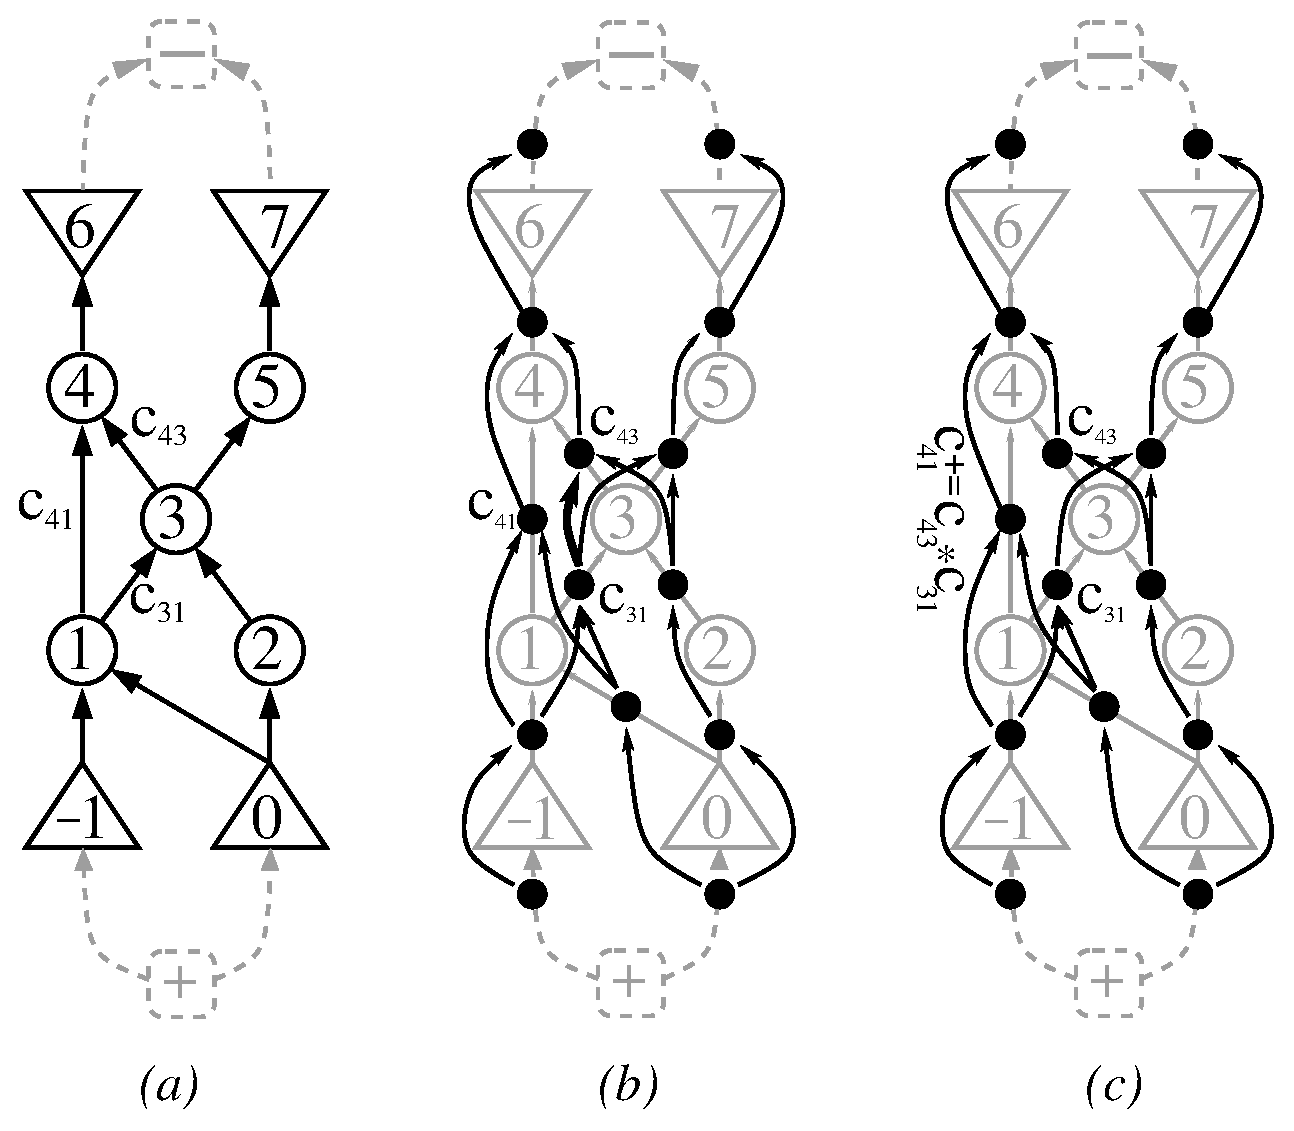
\includegraphics[width=.65\textwidth]{face_elims}
  \caption{
    (a) $G$ extended, 
    (b) $\cal G$ overlaid, 
    (c) face elimination 
  }
  \label{fig:face_elims}
\end{figure}
A complete face elimination sequence $\sigma_f$ yields a tripartite 
directed line graph $\sigma_f({\cal G})$ that can be transformed back into 
the bipartite graph representing the Jacobian $\bmfp$.
We note that any $G$ can be transformed into the 
corresponding $\cal G$ but that a back transformation 
generally is not  possible once face elimination steps have been applied. 
Therefore, face eliminations can generally not precede vertex and edge 
eliminations.
In \OpenAD\ these eliminations are implemented in the algorithms described in 
\refsec{sssec:MMTradeOff} and \refsec{sssec:angel}.

In a source transformation context of \OpenADF\ the operations \refeqn{eqn:fma} are 
expressed as actual code, the Jacobian accumulation code. For our example code 
from \reffig{fig:toyBB} the code computing 
the local partials in conjunction with the function value 
is shown in 
\reffig{fig:toyAndPartials}.
\footnote{
  For better readability we write the indices of the $c_{ji}$ with commas.
} 
\begin{figure}
  \begin{center}
    \begin{minipage}{.3\linewidth}
      \begin{align*}
        v_1&=v_{-1}+v_0; \\
        v_2&=\sin(v_0); \\
        v_3&=v_1+v_2; \\
        v_4&=v_1*v_3; \\
        v_5&=\sqrt{v_3};\\
        v_6&=\cos(v_4); \\
        v_7&=-v_5;
      \end{align*}
    \end{minipage}
    \begin{minipage}{.3\linewidth}
      \begin{align*}
        c_{1,-1}&=1; \\
        c_{2,0}&=\cos(v_0); \\
        c_{3,1}&=1; \\
        c_{4,1}&=v_3; \\
        c_{5,3}&=(2\sqrt{v_3})^{-1}; \\
        c_{6,4}&=-\sin(v_4); \\
        c_{7,5}&=-1;
      \end{align*}
    \end{minipage}
    \begin{minipage}{.2\linewidth}
      \begin{align*}
        c_{1,0}&=1; \\
        &\\
        c_{3,2}&=1; \\
        c_{4,3}&=v_1; \\
        &\\
        &\\
        &
      \end{align*}
    \end{minipage}
  \end{center}	
  \caption{Pseudo code for \refeqn{eqn:sampleCode} and the computation of the $c_{ji}$}\label{fig:toyAndPartials}
\end{figure}
In \OpenADF\ the operations in \reffig{fig:toyAndPartials} are generated by the 
transformation algorithm discussed in \refsec{sssec:linearization}.
The operations induced by the eliminations on the graph can 
be expressed in terms of the auxiliary variables $c_{ji}$.
For our example, a forward vertex elimination in the order  (1,2,3,4,5) 
in $G$ (\reffig{fig:elims}), leads to the
following Jacobian accumulation code.
\begin{figure}[h]
  % \begin{minipage}{\linewidth}
  %   \begin{align*}
  %     1:\quad  &c_{3,-1}=c_{3,1} * c_{1,-1};~c_{3,0}=c_{3,1} * c_{1,0};~c_{4,-1}=c_{4,1} * c_{1,-1};~c_{4,0}=c_{4,1} * c_{1,0}; \\
  %     2:\quad  &c_{3,0}=c_{3,2} * c_{2,0}+c_{3,0}; \\
  %     3:\quad  &c_{4,-1}=c_{4,3} * c_{3,-1}+c_{4,-1};~c_{4,0}=c_{4,3} * c_{3,0}+c_{4,0};~c_{5,-1}=c_{5,3} * c_{3,-1}; \\
  %     &c_{5,0}=c_{5,3} * c_{3,0}; \\
  %     4:\quad  &c_{6,-1}=c_{6,4} * c_{4,-1};~c_{6,0}=c_{6,4} * c_{4,0}; \\
  %     5:\quad  &c_{7,-1}=c_{7,5} * c_{5,-1};~c_{7,0}=c_{7,5} * c_{5,0} \quad .
  %   \end{align*}
  % \end{minipage}
  \begin{tabular}{l@{\hspace{1ex}}r@{\hspace{0.1ex}}l@{\hspace{1ex}}l@{\hspace{1ex}}l}
    1: &$c_{3,-1}$&$=c_{3,1} * c_{1,-1};         $&$c_{3,0}=c_{3,1} * c_{1,0};        $&$c_{4,-1}=c_{4,1} * c_{1,-1};$\\
    &$c_{4,0} $&$=c_{4,1} * c_{1,0};          $&                                    &                              \\
    2: &$c_{3,0} $&$=c_{3,2} * c_{2,0}+c_{3,0};  $&                                    &                              \\
    3: &$c_{4,-1}$&$=c_{4,3} * c_{3,-1}+c_{4,-1};$&$c_{4,0}=c_{4,3} * c_{3,0}+c_{4,0};$&$c_{5,-1}=c_{5,3} * c_{3,-1};$\\
    &$c_{5,0} $&$=c_{5,3} * c_{3,0};          $&                                    &                              \\
    4: &$c_{6,-1}$&$=c_{6,4} * c_{4,-1};         $&$c_{6,0}=c_{6,4} * c_{4,0};        $&                              \\
    5: &$c_{7,-1}$&$=c_{7,5} * c_{5,-1};         $&$c_{7,0}=c_{7,5} * c_{5,0};        $&            
  \end{tabular}
  \caption{Pseudo code for vertex eliminations for \refeqn{eqn:sampleCode}}\label{fig:toyAccumulation}
\end{figure}
In the tool the operations shown in \reffig{fig:toyAccumulation} are generated by the 
transformation algorithm discussed in \refsec{sssec:BBPreacc}. 
% -----------------------------------------------------------------------------------------
\subsection{Control Flow Reversal} \label{ssec:cfReversal}
Because the code for a $\bmf$ generally contains control flow constructs there is no 
single  computational graph 
$G$ that represents the computation of $\bmf$ for all possible values of $\bmx$.
We explained in \refsec{ssec:computationalGraphs} that \OpenADF\ considers subgraphs constructed 
from the contents of a \basicblock.
In the example shown in \reffig{fig:toy} we put the \basicblock\ code shown in 
\reffig{fig:toyBB} into a control flow context, see lines 06--09.
\begin{figure}
  \begin{center}
    \begin{minipage}{.5\textwidth}
      \begin{tabbing}
        \hspace{.6cm}{\footnotesize \bf 00}\hspace{.5cm} {\tt y(k) = sin(x(1)*x(2))} \\
        \hspace{.6cm}{\footnotesize \bf 01}\hspace{.5cm} {\tt k    = k+1} \\
        \hspace{.6cm}{\footnotesize \bf 02}\hspace{.5cm} {\tt if} \={\tt (mod(k,2) .eq. 1) then } \\
        \hspace{.6cm}{\footnotesize \bf 03}\hspace{.5cm} \>{\tt y(k) = 2*y(k-1)}  \\
        \hspace{.6cm}{\footnotesize \bf 04}\hspace{.5cm} {\tt else } \\
        \hspace{.6cm}{\footnotesize \bf 05}\hspace{.5cm} \>{\tt do} \={\tt i=1,k } \\
        \hspace{.6cm}{\footnotesize \bf 06}\hspace{.5cm} \>\>{\tt t1   = x(1)+x(2) } \\
        \hspace{.6cm}{\footnotesize \bf 07}\hspace{.5cm} \>\>{\tt t2   = t1+sin(x(1)) } \\
        \hspace{.6cm}{\footnotesize \bf 08}\hspace{.5cm} \>\>{\tt x(1) = cos(t1*t2) } \\
        \hspace{.6cm}{\footnotesize \bf 09}\hspace{.5cm} \>\>{\tt x(2) = -sqrt(t2) } \\
        \hspace{.6cm}{\footnotesize \bf 10}\hspace{.5cm} \>{\tt end do } \\
        \hspace{.6cm}{\footnotesize \bf 11}\hspace{.5cm} {\tt end if } \\
        \hspace{.6cm}{\footnotesize \bf 12}\hspace{.5cm} {\tt y(k) = y(k)+x(1)*x(2) } 
      \end{tabbing}
    \end{minipage}
  \end{center}
  \caption{Toy example code with control flow}\label{fig:toy}
\end{figure}
The control flow graph (CFG) \cite{ASU86} resulting from the above code is depicted in 
\reffig{fig:cfg}(a).
The assignment statements are contained in the {\basicblock}s B(2,4,6,9).
For instance, 
the statements from \reffig{fig:toyBB} now  in lines 06--09 form the loop body, \basicblock\ B(6).
As B(6) is executed
\code{k} times it may be worth putting
additional effort into the optimization of the derivative code 
generated for B(6) by optimizing the elimination sequence as illustrated in 
\refsec{ssec:elimMeth}.
\begin{figure}[ht]
  \centering
  \begin{tabular}{ccc}
    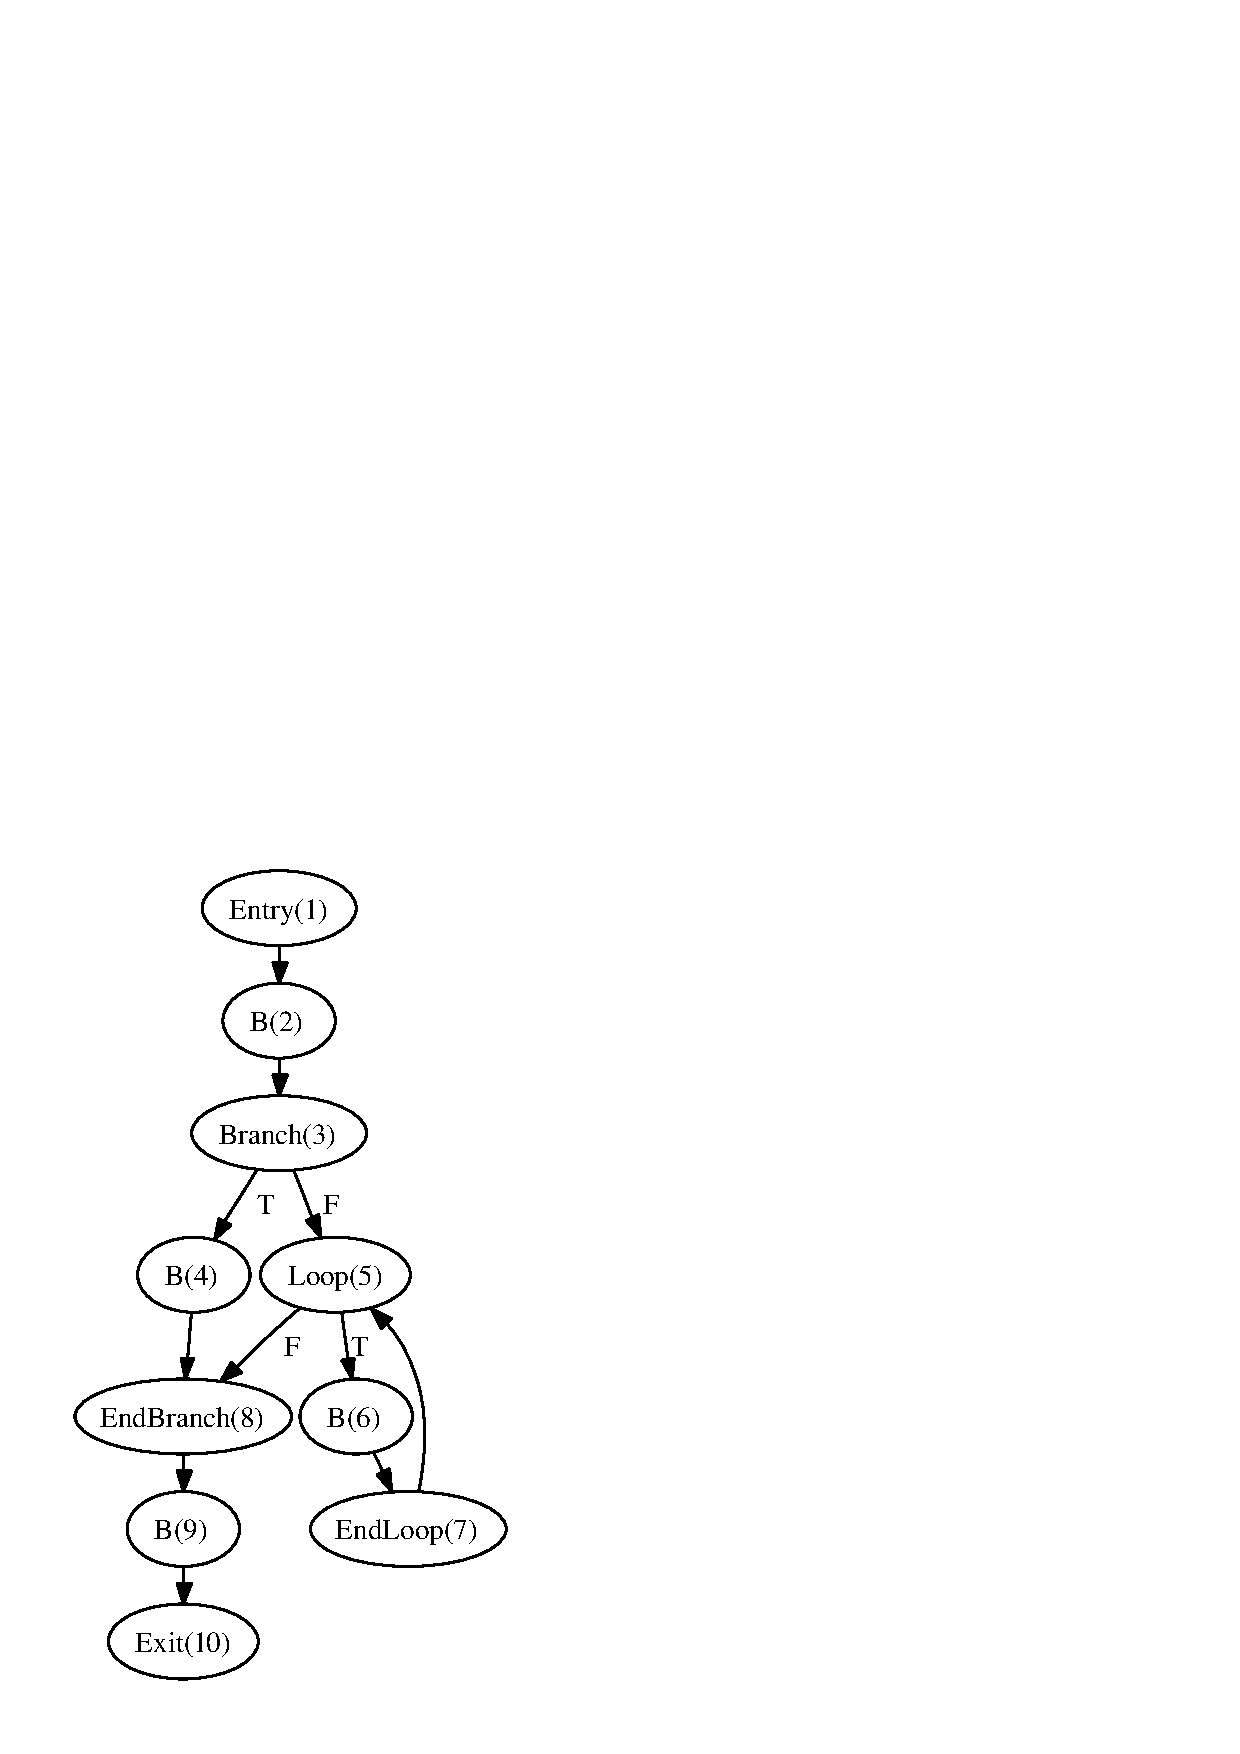
\includegraphics[width=.25\textwidth]{cfg_ts}
    &
    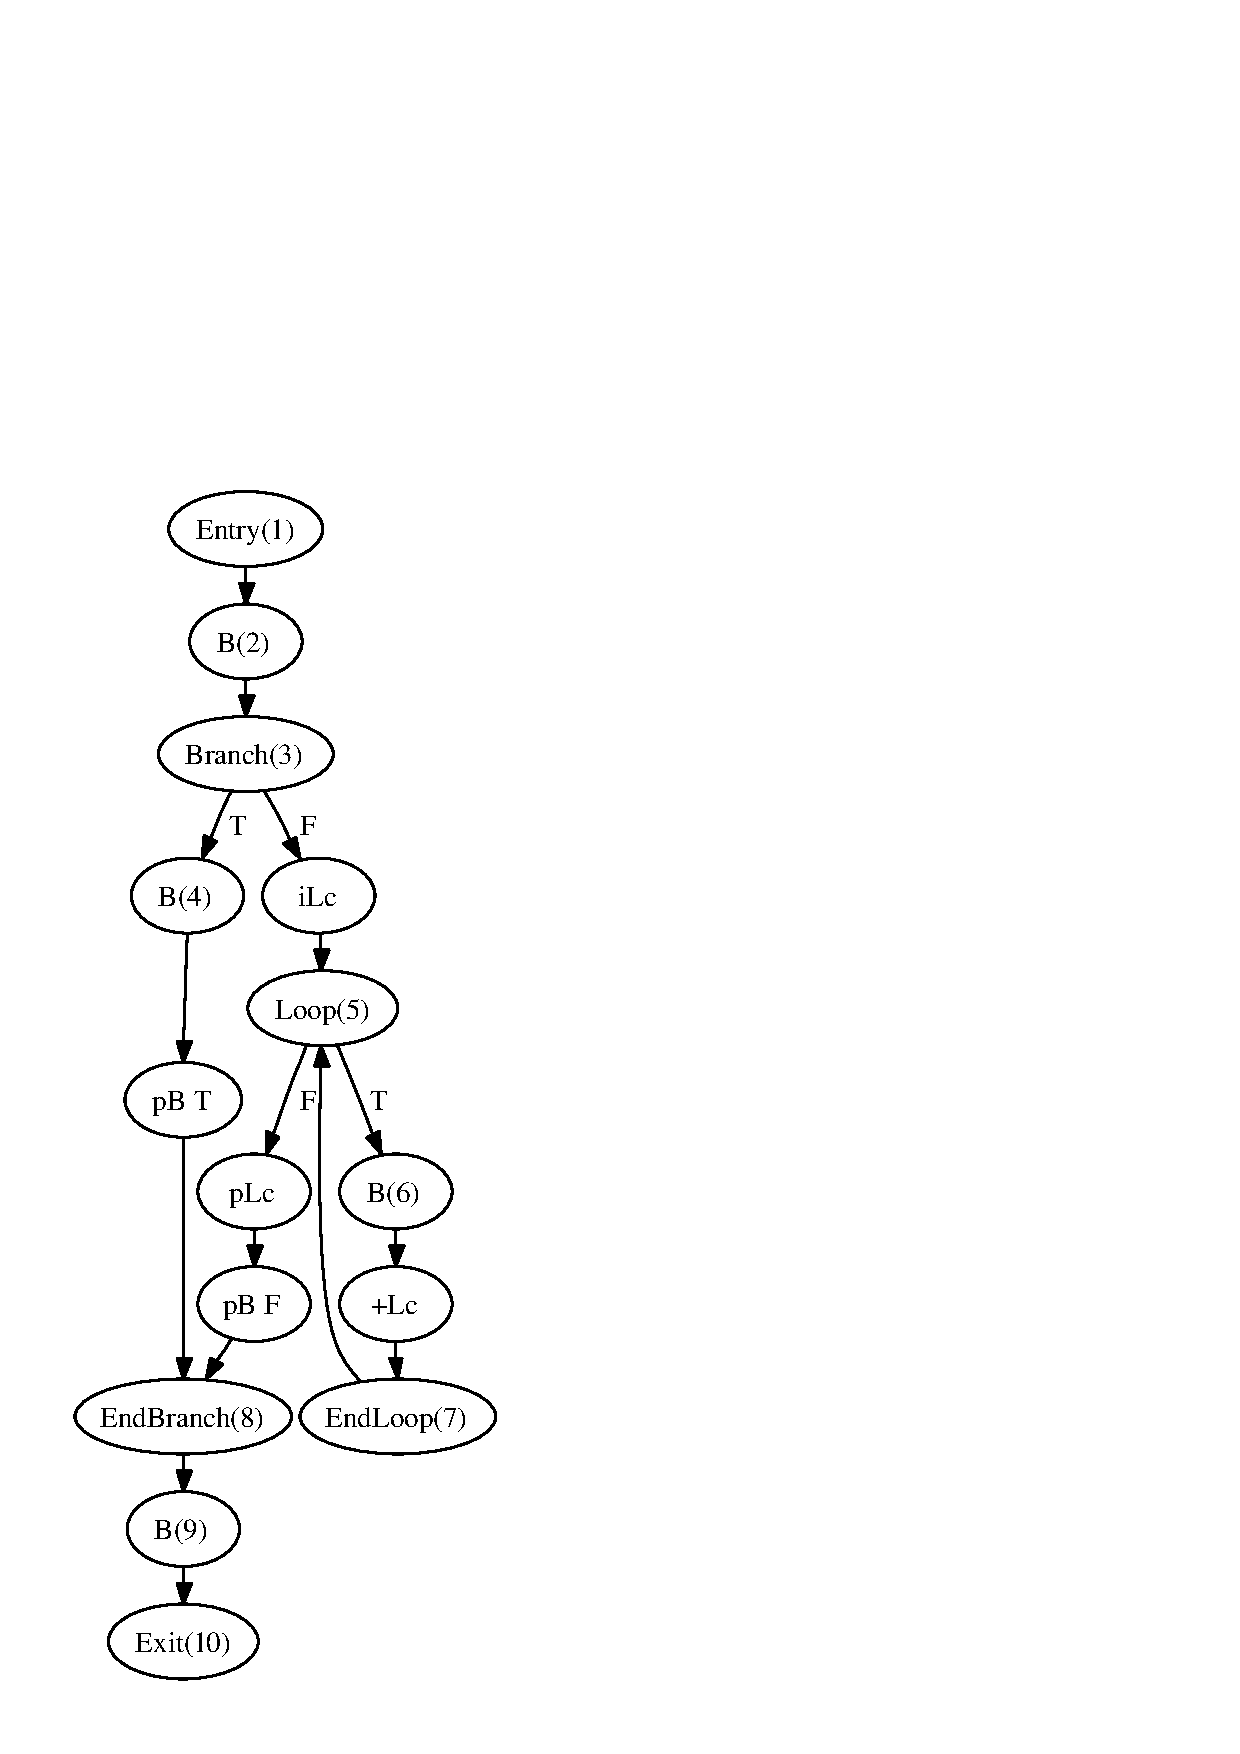
\includegraphics[width=.25\textwidth]{cfg_tape}
    &
    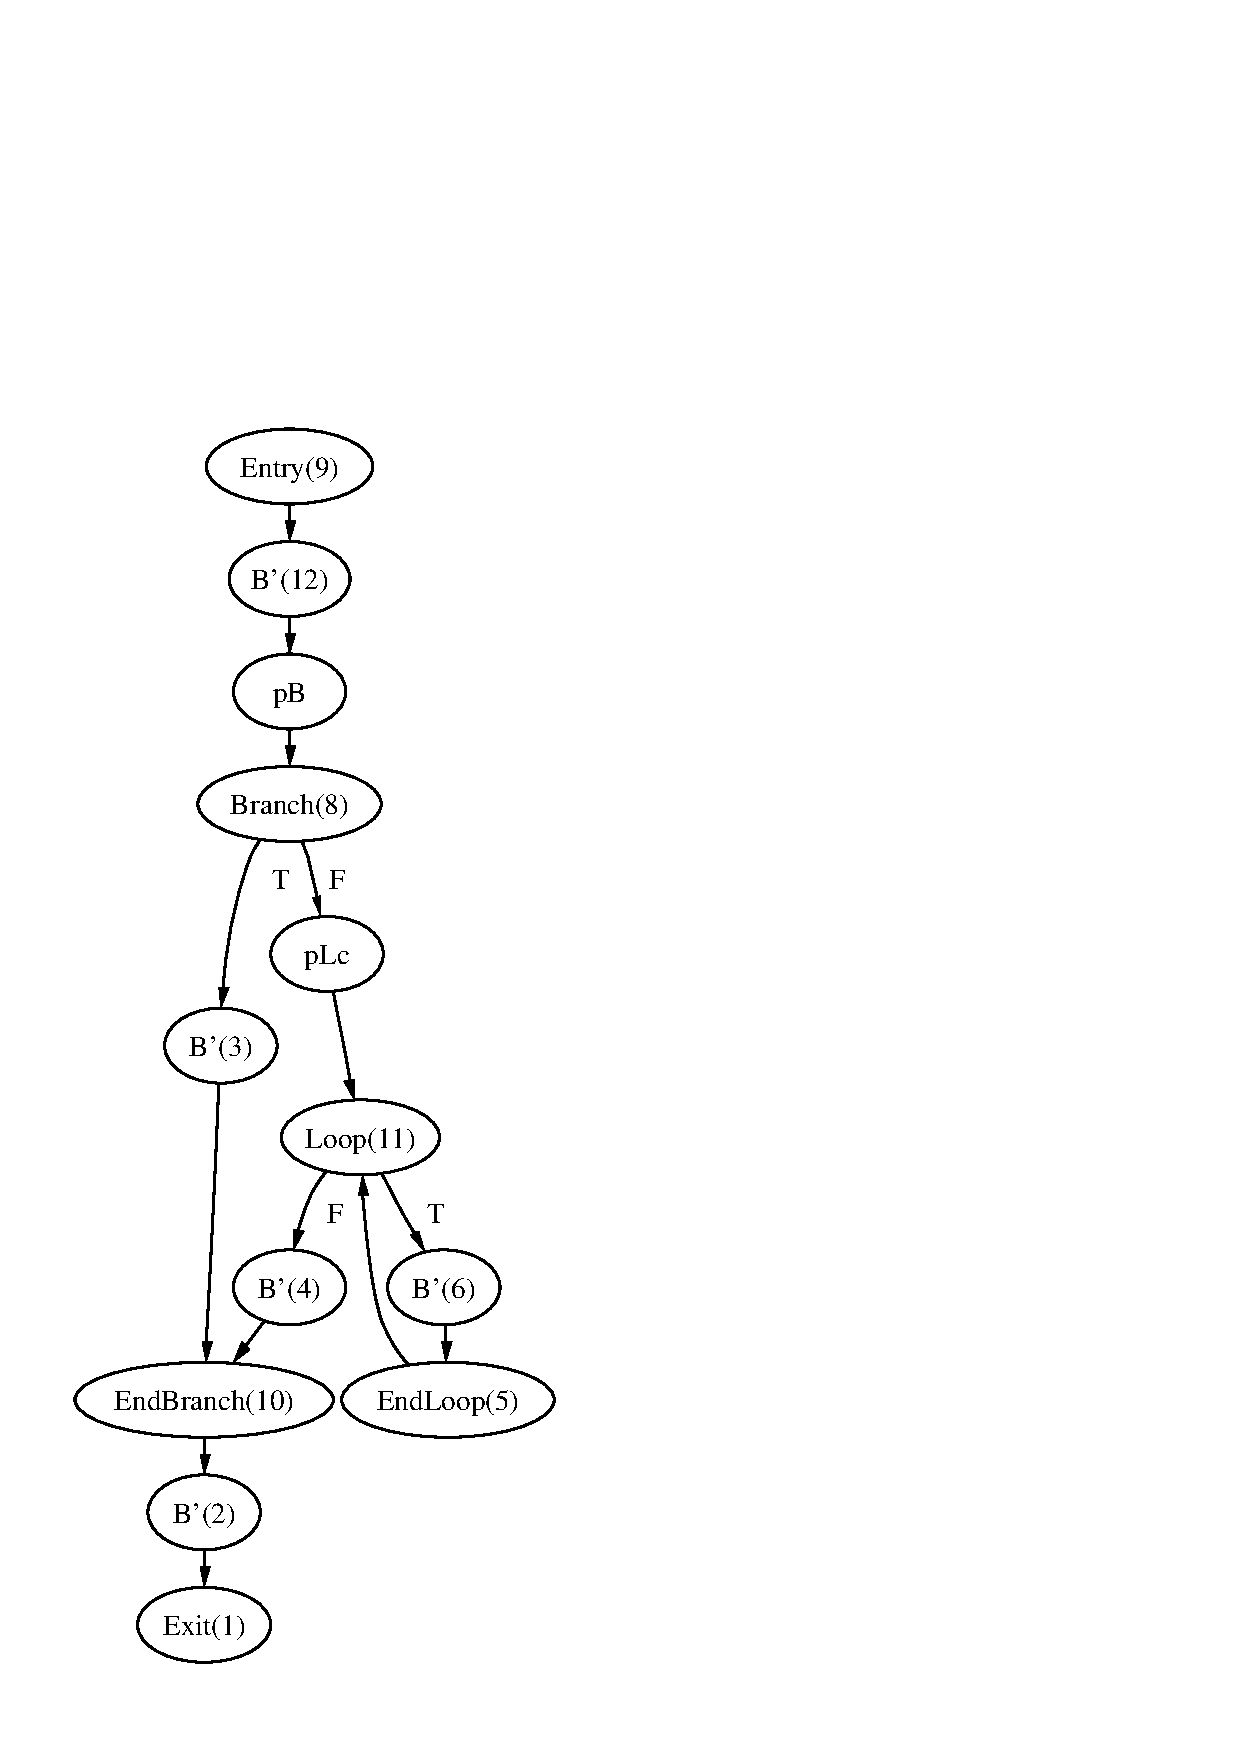
\includegraphics[width=.25\textwidth]{cfg_adj}
    \\
    \em (a) & \em (b) & \em (c)
  \end{tabular}
  \caption{CFG of \reffig{fig:toy} (a) original, (b) trace generating, (c) reversed}\label{fig:cfg}
\end{figure}
For B(6) the corresponding computational graph $G$  see 
\reffig{fig:elims}(a).  

For a sequence of $l$ {\basicblock}s that are part of 
a path through the CFG for a particular value of $\bmx$ the 
equations~(\ref{eqn:fm}) and (\ref{eqn:rm}) can be generalized as follows:
\begin{equation} \label{eqn:bbfm}
  \dot{\bmy}_j=\bmJ_j \dot{\bmx}_j \quad \text{for}~~j=1,\ldots,l
\end{equation} 
and 
\begin{equation} \label{eqn:bbrm}
  \bar{\bmx}_j=\bmJ^T_j \bar{\bmy}_j \quad \text{for}~~j=l,\ldots,1\quad ,
\end{equation} 
where $\bmx_j = (x^j_i \in V :  i=1,\ldots,n_j)$ and
$\bmy_j = (y^j_i \in V : i=1,\ldots,m_j)$ are the inputs and outputs of the 
{\basicblock}s
respectively. 
In {\em forward mode} a sequence of 
products of the local Jacobians $\bmJ_j$ 
with the directions $\dot{x}_j$ 
are propagated forward in the direction of the flow of control, for 
instance simultaneouly to the computation of $\bmf$.
In our example \basicblock\ B(6) is the third \basicblock\ ($j=3$) and we have
$\bmx_3=\bmy_j=($\code{x(1)}$,$\code{x(2)}$)$ and 
consequently have the operations for the Jacobian vector product shown 
in \reffig{fig:JacVec}.  
\begin{figure}[h]
  \begin{center}
    \begin{align*}
      t_1&=\dot{\tt x}\mbox{\tt (1)} ; \\
      t_2&=\dot{\tt x}\mbox{\tt (2)}; \\
      \dot{\tt x}\mbox{\tt (1)}&=c_{6,-1}*t_1; \\
      \dot{\tt x}\mbox{\tt (1)}&=\dot{\tt x}\mbox{\tt (1)}+c_{6,0}*t_2; \\
      \dot{\tt x}\mbox{\tt (2)}&=c_{7,-1}*t_1; \\
      \dot{\tt x}\mbox{\tt (2)}&=\dot{\tt x}\mbox{\tt (2)}+c_{7,0}*t_2; 
    \end{align*}
  \end{center}	
  \caption{Pseudo code for $\bmJ_3\dot{\bmx}_3$ for the loop body in \reffig{fig:toy}}\label{fig:toyPreacc}
\end{figure}
Note that the code overwrites \code{x(1)} and \code{x(2)} and therefore 
we have to preserve the original derivatives in temporaries $t_1$ and $t_2$.

In {\em reverse mode} products of the transposed
Jacobians $\bmJ^T_j$ with adjoint vectors $\overline{\bmy}_j$
are propagated reverse to the direction of the flow of control.
The $\bmJ^T_j$ can be computed by augmenting the original code with 
linearization and Jacobian accumulation statements, see \refsec{ssec:elimMeth}.
The preaccumulated  $\bmJ^T_j$ are stored during the forward execution
which is commonly called the {\em tape}..They are retrieved from the 
tape for computing \refeqn{eqn:bbrm} during the reverse execution. 
It is possible to organize the store and retrieve such that the tape can be 
implemented as a stack.
\begin{figure}[h]
  \begin{center}
    \begin{minipage}[b]{.2\linewidth}
      \code{push(}$c_{6,-1}$\code{);}\\
      \code{push(}$c_{6,0}$\code{);}\\
      \code{push(}$c_{7,-1}$\code{);}\\
      \code{push(}$c_{7,0}$\code{);}\\
      \\ \\ \\
      \centerline{(a)}
    \end{minipage}
    \begin{minipage}[b]{.2\linewidth}
      \small
      \begin{align*}
        t_2&=\code{pop()}*\bar{\tt x}\mbox{\tt (2)};\\
        t_1&=\code{pop()}*\bar{\tt x}\mbox{\tt (2)};\\
        t_2&=t_2+\code{pop()}*\bar{\tt x}\mbox{\tt (1)};\\
        t_1&=t_1+\code{pop()}*\bar{\tt x}\mbox{\tt (1)};\\
        \bar{\tt x}\mbox{\tt (2)}& =t_2;\\
        \bar{\tt x}\mbox{\tt (1)}& =t_1;
      \end{align*}
      \centerline{(a)}
    \end{minipage}
  \end{center}	
  \caption{Pseudo code for writing the tape (a) and consuming the tape for  $\bmJ_3^T\bar{\bmy}_3$ (b) for  the loop body in \reffig{fig:toy}}\label{fig:toyPreacc}
\end{figure}

In order to find the corresponding path to the reversed control flow graph 
we also have to generate a trace which is done with an augmented CFG,
for our toy example see \reffig{fig:cfg}(b).
This augmented CFG  keeps track of which branch was taken and counts how 
often a loop was 
executed.  
This information is pushed on  a stack and popped from that stack during the 
reverse sweep see also \cite{scam2004}. Because the control flow trace 
adheresto the stack model it often is also considered part of the tape. 
In the example in \reffig{fig:cfg}(b) the extra {\basicblock}s pBT and pBF push 
a boolean (T or F) onto the stack depending on the branch. 
In iLc we initialize a loop counter, increment the loop counter in +Lc, 
and push the final count in pLc. 

\reffig{fig:cfg}(c) shows the reversed CFG for our toy example. 
The parenthesized numbers in the node labels align the 
node transformation to \reffig{fig:cfg}(a). 
The \exit\ node becomes 
the \entry, \Loop\ becomes \EndLoop, \branch\ beomes \EndBranch, and vice versa. 
Each \basicblock\  B is replaced with its reversed version B'.  
Finally, to find the proper path through this reversed CFG we need to retrieve 
the information recorded in  \reffig{fig:cfg}(b). The extra nodes pB and pLc 
pop the branch information and the loop counter respectively.  
We enter the branch and execute the loop as indicated by the recorded information. 
The process of the control flow reversal is described in detail in 
\cite{NULF04CFR}. 

% -----------------------------------------------------------------------------------------
\subsection{Call Graph Reversal} \label{ssec:cgReversal}

Generally, the computer program 
induces a {\em call graph} (CG) \cite{ASU86}
whose vertices are subroutines and whose edges 
represent calls potentially made during the computation of $\bmy$ for all 
values of $\bmx$ in the domain of $\bmf$.

For a large number of problems it is possible to statically 
predetermine either 
{\em split} or {\em joint} 
reversal /cite{grie00} for any subroutine in the call graph .
These concepts are easier understood with the help of the dynamic call tree,
see also \cite{iccs2005}.
\begin{figure}
  \centering
  \begin{tabular}{p{.5\linewidth}p{.3\linewidth}}
    \begin{minipage}[b]{\linewidth}
      \footnotesize
      \tt subroutine A()\\
      \hspace*{3ex}call B(); call D(); call B();\\
      end subroutine A\\[.2em]
      subroutine B()\\
      \hspace*{3ex}call C()\\
      end subroutine B\\[.2em]
      subroutine C()\\
      \hspace*{3ex}call E()\\
      end subroutine C
    \end{minipage}
    &
    \vspace*{-3.2cm}
    \centering{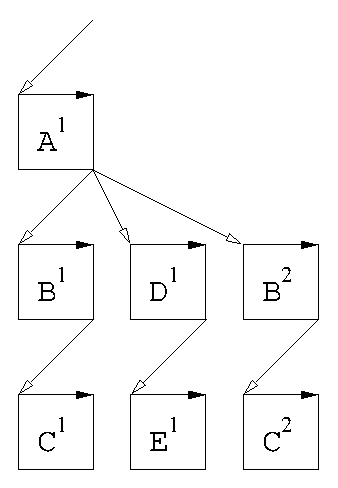
\includegraphics[width=3.2cm,origin=c,angle=-90]{edct_ns}}
  \end{tabular}
  \caption{Dynamic call tree of a simple calling hierarchy}
  \label{fig:simple_dct}
\end{figure}
where ach vertex represents an actual invocation of a subroutine for a 
given execution of the program, see \reffig{fig:simple_dct} and 
\reftab{tab:leg} for an explanation of the symbols. 
The order of calls is implied by following the edges in left to right order. 
Using split reversal for all subroutines in the  program 
means that first the tape for the entire program is written. Then 
we follow with the reverse steps that read the tape, see \reffig{fig:split}. 

\begin{table}[t]
  \begin{center}
    \begin{tabular}{clcl}
      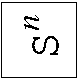
\includegraphics[origin=c,angle=-90,width=0.7cm]{box}  
      & 
      \begin{minipage}[b]{.3\linewidth}
        $n$-th invocation
        of subroutine {\tt S}
      \end{minipage} 
      & 
      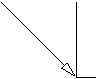
\includegraphics[origin=c,angle=-90,width=0.7cm]{call} & 
      \begin{minipage}[b]{.3\linewidth}
        subroutine call\\[-2mm]
      \end{minipage} 
      \\ 
      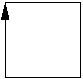
\includegraphics[origin=c,angle=-90,width=0.7cm]{rf}  & 
      \begin{minipage}[b]{.3\linewidth}
        run forward \\[-2mm]
      \end{minipage}
      & 
      
\includegraphics[origin=c,angle=-90,width=0.7cm]{order}  & 
      \begin{minipage}[b]{.3\linewidth}
        order of execution \\[-2mm]
      \end{minipage}
      \\
      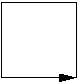
\includegraphics[origin=c,angle=-90,width=0.7cm]{sac}  & 
      \begin{minipage}[b]{.3\linewidth}
        store checkpoint \\[-2mm]
      \end{minipage}
      & 
      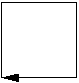
\includegraphics[origin=c,angle=-90,width=0.7cm]{rac}  & 
      \begin{minipage}[b]{.3\linewidth}
        restore checkpoint \\[-2mm]
      \end{minipage}
      \\
      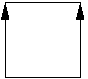
\includegraphics[origin=c,angle=-90,width=0.7cm]{ta}  & 
      \begin{minipage}[b]{.3\linewidth}
        run forward and tape \\[-2mm]
      \end{minipage}
      & 
      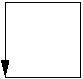
\includegraphics[origin=c,angle=-90,width=0.7cm]{ad}  & 
      \begin{minipage}[b]{.3\linewidth}
        run adjoint \\[-2mm]
      \end{minipage}
      \\
    \end{tabular}
  \end{center}
  \vspace*{-.5cm}
  \caption{Symbols for call tree reversal}
  \label{tab:leg}
\end{table}

\begin{figure}[t]
  \centerline{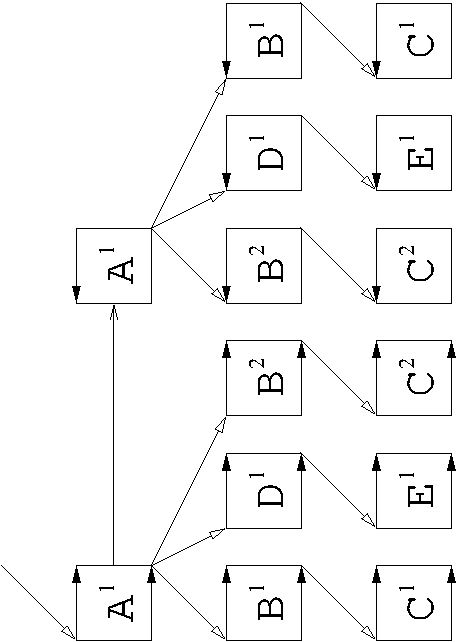
\includegraphics[width=3.2cm,origin=c,angle=-90]{edct_split_ns}}
  \vspace*{-.5cm}
  \caption{Dynamic call tree for split reversal}
  \label{fig:split}
\end{figure}

\begin{figure}[t]
  \centerline{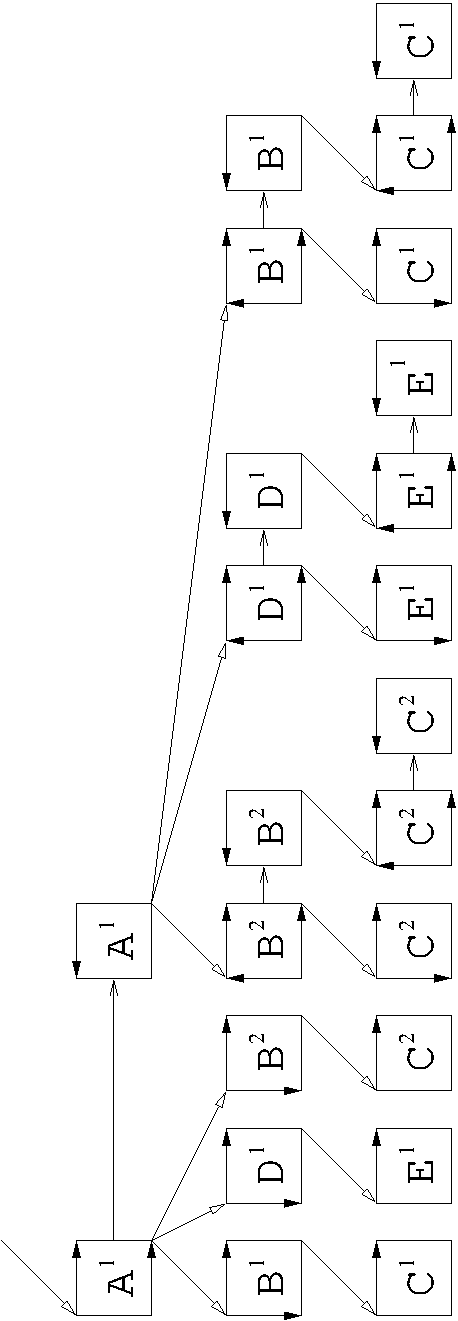
\includegraphics[width=3.2cm,origin=c,angle=-90]{edct_joint_ns}}
  \vspace*{-3cm}
  \caption{DCT of adjoint obtained by joint reversal mode}
  \label{fig:joint}
\end{figure}

Using joint reversal for all subroutines in a program 
means that the tape, see \refsec{ssec:cfReversal} for a each 
subroutine invocation is written immediately before the reverse execution for 
that invocation. In our example this implies that we have to generate 
a tape for {\tt C}$^2$ while the caller {\tt B}$^2$ is being reversed, 
i.e. this is not the proper context to simply reexecute {\tt C}$^2$. 
We can either reexecute the entire program up to the  {\tt C}$^2$
call and then start taping, or (preferrably) we store the arguments while 
running forward and restore them before starting the taping. 
The ensuing dynamic call tree for our example is 
shown in \reffig{fig:joint}. 
For many applications neither an all split nor all joint reversal
is efficient. Often a mix of split and joint reversals statically  
applied to subtrees of the call tree is suitable.  

% #########################################################################################
\section{Components of \OpenADF}\label{sec:openadfcomponents}

\OpenADF\ is built on components that belong to a framework designed
for code transformation of numerical programs.  The components are
tied together either via programmatic interfaces or by communication
using the \xaif\ langauge. The transformation of the source code follows the
pipeline shown in \reffig{fig:overview}.  
In \refsec{ssec:openadcomponents} we describe the language-indepdendent 
components of \OpenAD\ framework and \refsec{ssec:fortfe} provides details 
in the Fortran front-end.
The regular setup procedure for \OpenADF, see also \refsec{ssec:dab}, 
will retrieve all componenents into an \code{OpenAD/} directory to which 
we refer from here on.  

% -----------------------------------------------------------------------------------------
\subsection{Language Independent Components (\OpenAD)}\label{ssec:openadcomponents}

The component design of the tool aims for reuse of the different components 
for different types of source transformation of numerical codes, for 
different programming languages in which these tools are written and finally 
also for the reuse of the individual components in different contexts. 
A second, equally important concern is the flexibility of the tool.  
This section covers the language independent components that make up the core \OpenAD\ framework. 

% -----------------------------------------------------------------------------------------
\subsubsection{Static Code Analyses (\OpenAnalysis)} \label{sssec:openanalysis}

The \OpenAnalysis\ toolkit, see \cite{oaWeb}, separates program
analysis from language-specific or front-end specific intermediate
representations.  This separation enables a single implementation of
domain-specific analyses such as activity analysis, to-be-recorded
analysis, and linearity analysis in \OpenADF.  Standard analyses
implemented within \OpenAnalysis\ such as CFG construction, call graph
construction, alias analysis, reaching definitions, ud- and du-chains,
and side-effect analysis are also available via
\OpenADFortTk.

\OpenADFortTk\ interfaces with \OpenAnalysis\ as a producer and a
consumer.  A description of Alias analysis illustrates this
interaction.  \xaif\ requires an alias map data structure, in which
each variable reference is mapped to a set of virtual locations that
it may or must reference.  For example, if a global variable \code{g}
is passed into subroutine \code{foo} through the reference parameter
\code{p}, variable references \code{g} and \code{p} will reference the
same location within the subroutine \code{foo} and therefore be aliases.  
\OpenAnalysis\ determines the aliasing relationships by querying an
abstract interface called the alias IR interface, which is a 
language-independent interface between \OpenAnalysis\ and any
intermediate representation for an imperative programming language.  
An implementation of the alias IR interface for the Fortran~90
intermediate representation is part of
\OpenADFortTk.  The interface includes queries for an iterator over
all the procedures, statements in those procedures, memory references
in each statement, and memory reference expression and location
abstractions that provide further information about memory references
and symbols.  The results of the alias analysis are then provided back
to \OpenADFortTk\ through an alias results interface.

Using language-independent interfaces between \OpenAnalysis\ and the
intermediate representation will enable alias analysis for multiple
language front-ends without requiring \xaif\ to include the union of
all language features that affect aliasing (ie. pointer arithmetic and
casting in C/C++ and equivalence in Fortran~90).  Instead
\OpenAnalysis\ has analysis-specific interfaces for querying
language-specific intermediate representations.

\OpenAnalysis\ also performs activity analysis.  For activity analysis
the independent and dependent variables of interest are communicated
to the front-end through the use of pragmas, see \refsec{sssec:mfef}.
The results of the analysis are then encoded by the Fortram~90
front-end into \xaif.  The analysis indicates which variables are
active at any time, which memory references are active, and which
statements are active.

The activity analysis itself is based on the formulation in~\cite{HNP02}.
The main difference is that the data-flow framework in \OpenAnalysis\ does not
yet take advantage of the structured data-flow equations.  Activity analysis is
implemented in a context-insensitive, flow-sensitive interprocedural fashion.

All sources for \OpenAnalysis\ can be found under \code{OpenAD/OpenAnalysis/}.
% -----------------------------------------------------------------------------------------
\subsubsection{Representing the Numerical Core (\xaif)} \label{sssec:xaif}
{\color{red} JU: rewritten } 

To obtain a language independent representation of programs across multiple 
programming languages one might choose the union of all language features. 
On the other hand one can observe that the majority of differences between 
languages does not lie with the elemental numerical operations that are at the 
heart of AD transformations. This more narrow representation 
is a compromise permitting just enough coverage to achieve language 
independence for the numerical core across languages.
Consequently, certain program features are not represented and have 
to be retained by the language specific front-end to reassemble the 
complete program from the (transformed) numerical core.
Among the generic language features not considered part of the numerical core are: 
\begin{itemize}
  \parskip = -2pt
\item user type definitions and member access, see also \refsec{sssec:Canonicalization}
\item pointer arithmetic
\item I/O operations  
\item memory management, see also \refsec{sec:concl}
\item preprocessor directives
\end{itemize}
For a more general discussion regarding this compromise see also \cite{sea2000something}.
It is apparent that certain aspects of the adjoint code such as 
checkpointing, see \refsec{ssec:cgReversal}, and taping, see \refsec{ssec:cfReversal},
can involve memory allocation and various I/O schemes and therefore 
are not amenable to representation in the \xaif. 
At the same time it is also clear that the way  one has to handle the memory and I/O for 
taping and checkpointing is primarily determined by the problem size at runtime and not
primarily by the code we transform.   
Therefore in \OpenAD\ such transformation results are handled by  specific 
code expansion for subroutine specific templates and inlinable subroutine calls 
in the post processor, see \refsec{sssec:PostProcessor}. This not only avoids 
the typically language specific I/O and memory management aspects, it also 
affords additional flexibility.   

The format of choice in \OpenAD\ is an XML-based \cite{xmlWeb} hierarchy of 
directed graphs, referred to as \xaif 
\cite{HNN02}. Using XML is motivated by the existence of XML parsers and 
the ability to specify the \xaif\ specific XML contents with a schema which 
the parser can use to validate a given \xaif\ representation. 
The current \xaif\ schema is documented at \cite{xaifweb}.
The basic building blocks are the same data structures commonly found 
in compilers from top down call graph with scopes and symbol tables, 
control flow graphs as call graph vertices, basic blocks  as control flow 
graph vertices, statement lists contained in basic blocks, 
assignments as a statement with expression graphs,  and variable references 
and intrinsic operations as expression graph vertices. 
The role of the respective elements in the \xaif\ schema is fairly self evident. 
Elements are associated by containment. In the graph structures edges 
refer to source and target vertices by vertex ids. 
Variable references contain references to symbols which in turn 
are associated to symbol table elements via a scope and a symbol id. 
An example can be found in \refsec{sssec:wtxxtw}, \reffig{fig:exampleXaifCode}.
Further documentation for individual elements can be found directly in the 
schema annotations. 

The \xaif\ also contains the results of the code analyses provided 
by \OpenAnalysis, see \refsec{sssec:OpenAnalysis}. Some are exressed 
either as additional attributes on certain \xaif\ elements, e.g. for activity information. 
Side-effect analysis provides lists of variable references per subroutine, i.e. a call graph vertex element.
DuUd chains are expressed as list of ids found in the assignment \xaif\ element.
Alias information is epxressed as set of virtual addresses. 
DuUd chains and alias information is collected in maps indexed by keys associated with the call 
graph. References to individual entries held in these maps are expressed via foreign key 
attributs in the elements. 

The source transformation at the code of \OpenAD\ potentially changes and augments 
all elements of the \xaif. While it would in principle be possible  
to express the result entirely in the plain \xaif\ format we already mentioned the 
code expansion approach. Therefore the transformed \xaif\ adheres to a schema 
that is extended by a construct to represent inlinable subroutine calls and 
a specific list of control flow graphs that the post processor places in predefined 
locations in the subroutine template.    

The \xaif\ schema and examples can be found under \code{OpenAD/xaif/}.

% -----------------------------------------------------------------------------------------
\subsubsection{Transforming the Numerical Core (\xaifBooster)} \label{sssec:xaifBooster}
The transformation engine that differentiates the \xaif\ representation of 
$\bmf$ is called \xaifBooster. It is implemented in C++ based on a 
data structure that represents all information supplied in the \xaif\ input 
together with collection of algorithms that operate on this data structure, modify 
it and produce transformed \xaif\ output as the result. All sources for \xaifBooster\ can be found under \code{OpenAD/xaifBooster/}. The principal setup of the source tree is shown in \reftab{tab:dirStruct}.
\begin{figure}
  \centering 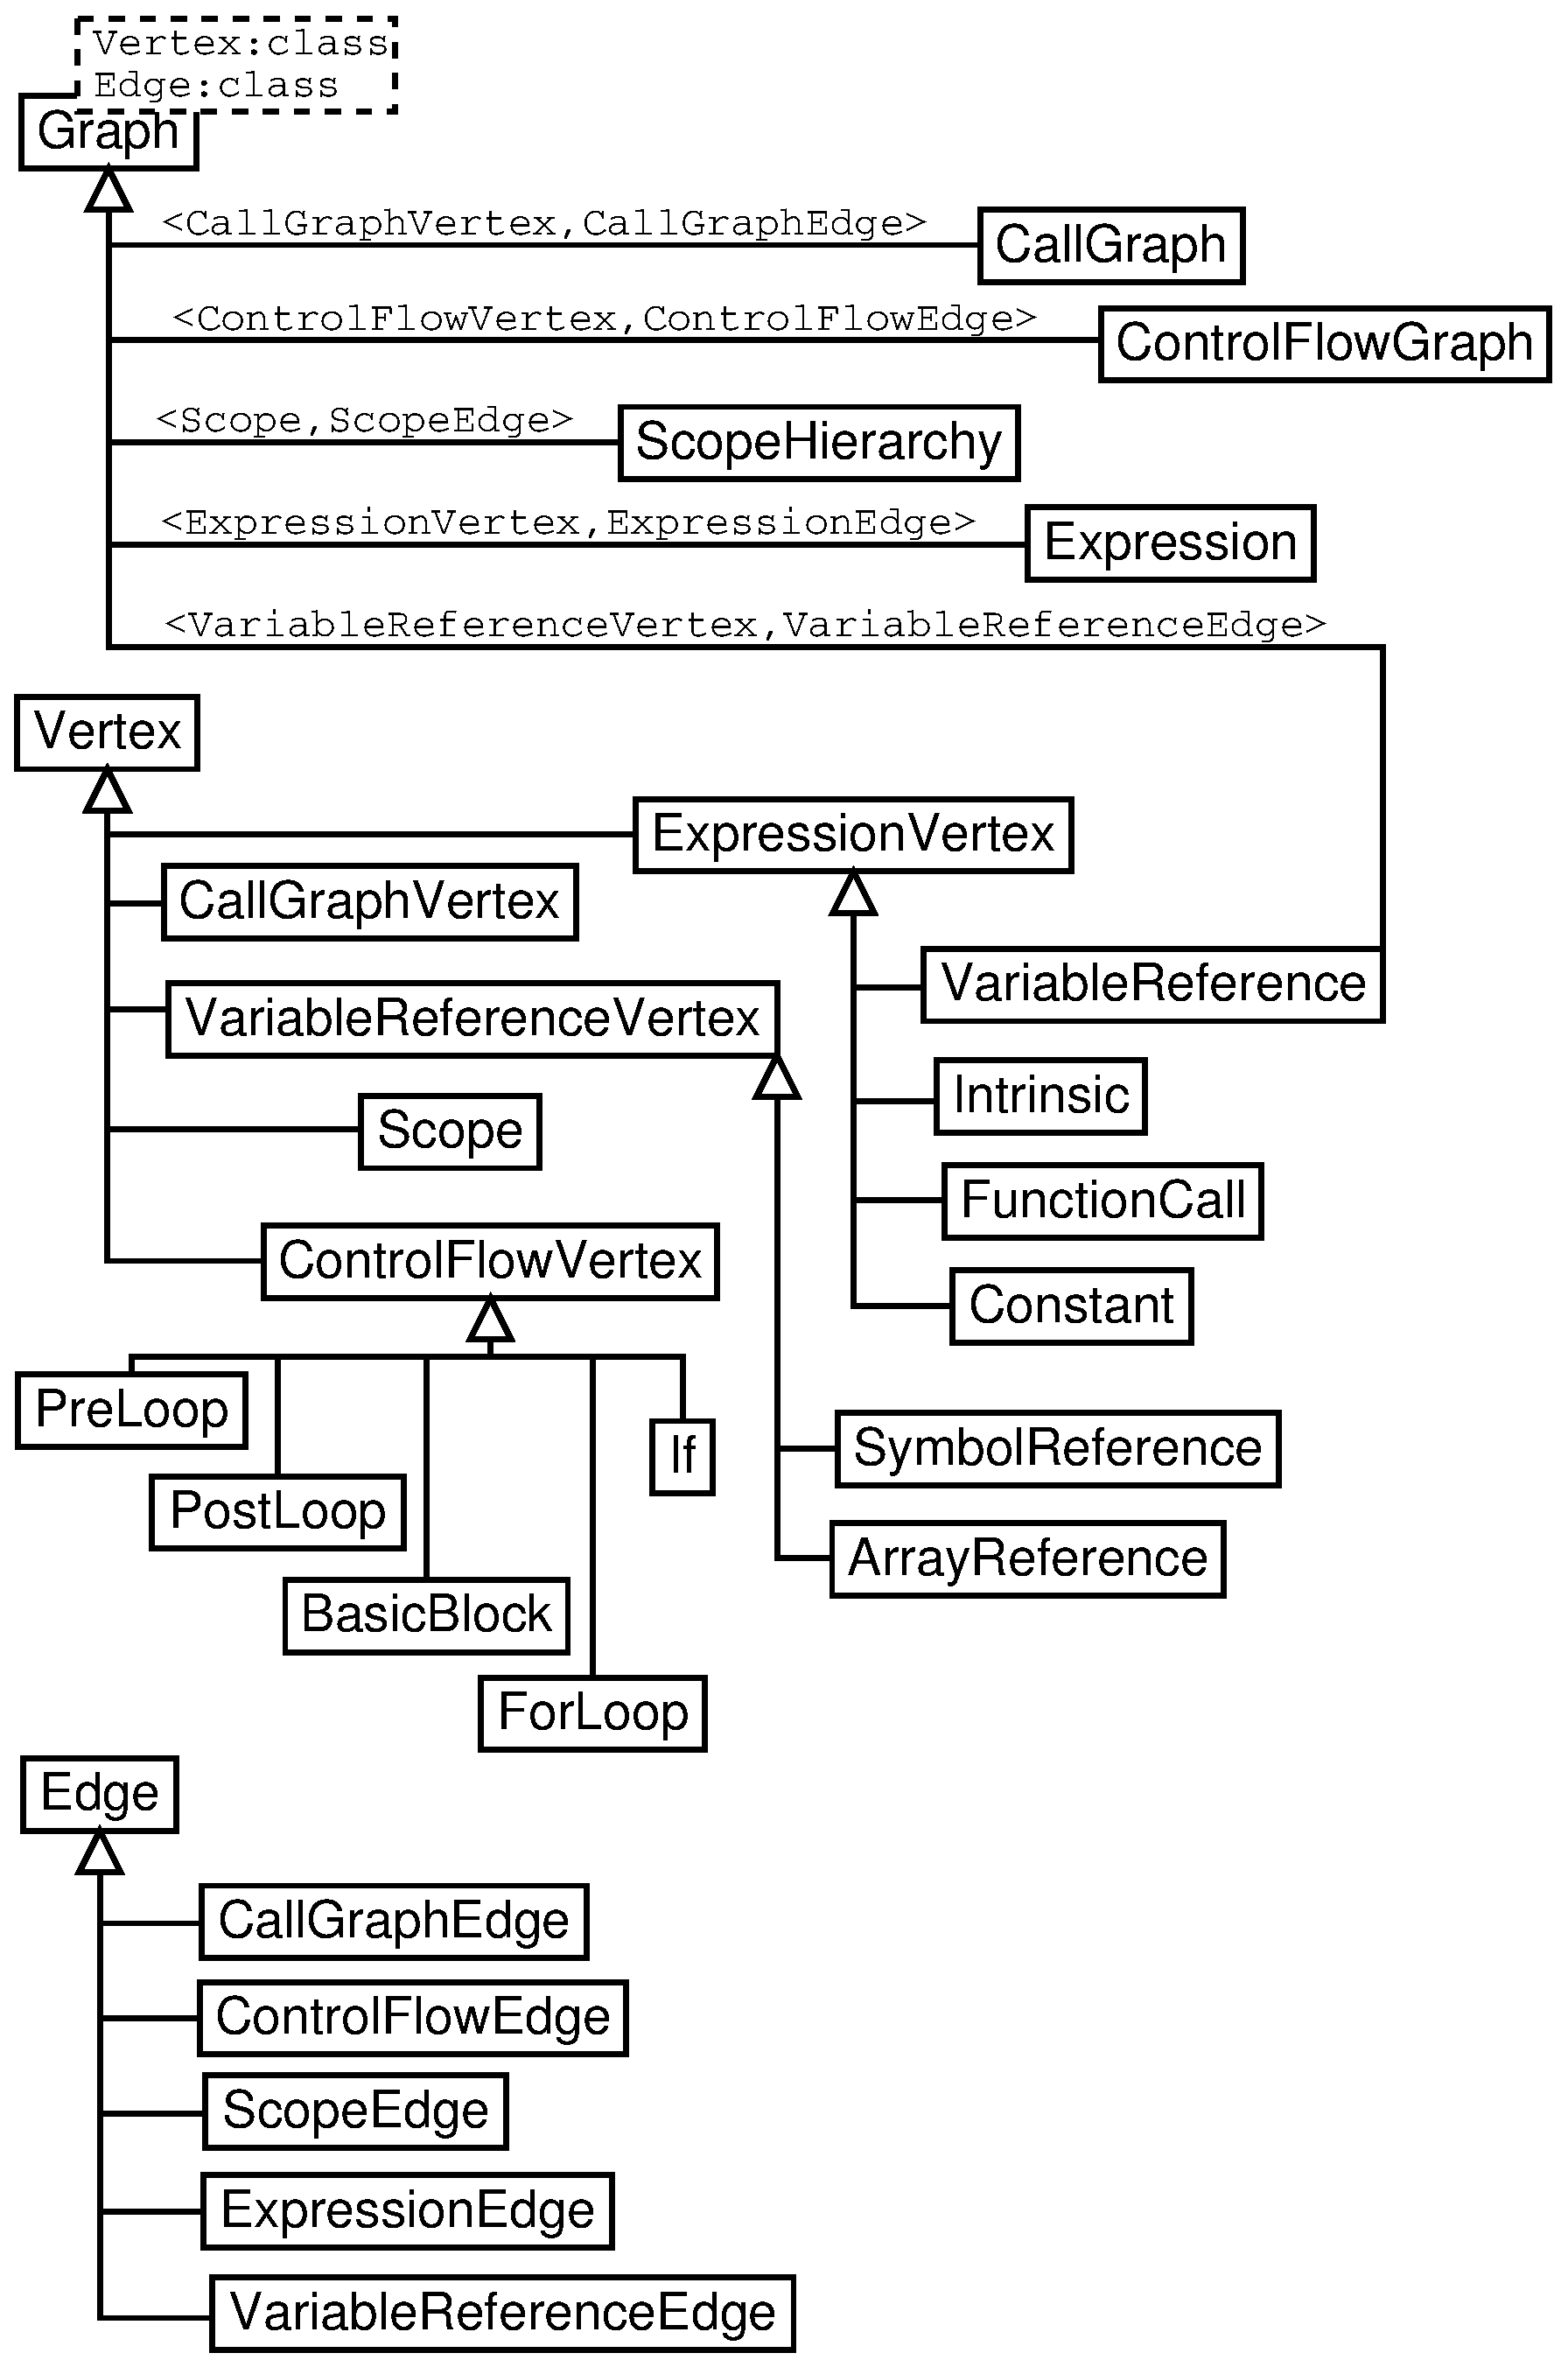
\includegraphics[width=.45\textwidth]{irInh}
  \caption{Simplified class inheritance in \xaifBooster} \label{fig:iri}
\end{figure}
The \xaifBooster\ data structure  
closely resembles the information one would find in a 
compiler's high level internal representation. 
the boost graph library \cite{boostWeb}
and the Standard C++ Library\cite{libstdcWeb}.
\reffigBS{fig:iri} and \reffig{fig:irc} show simplified subsets of the classes 
occuring in the \xaifBooster\ data structure in the inheritance 
as well as the composition hierarchy.  
\begin{figure}[htb]
  \centering 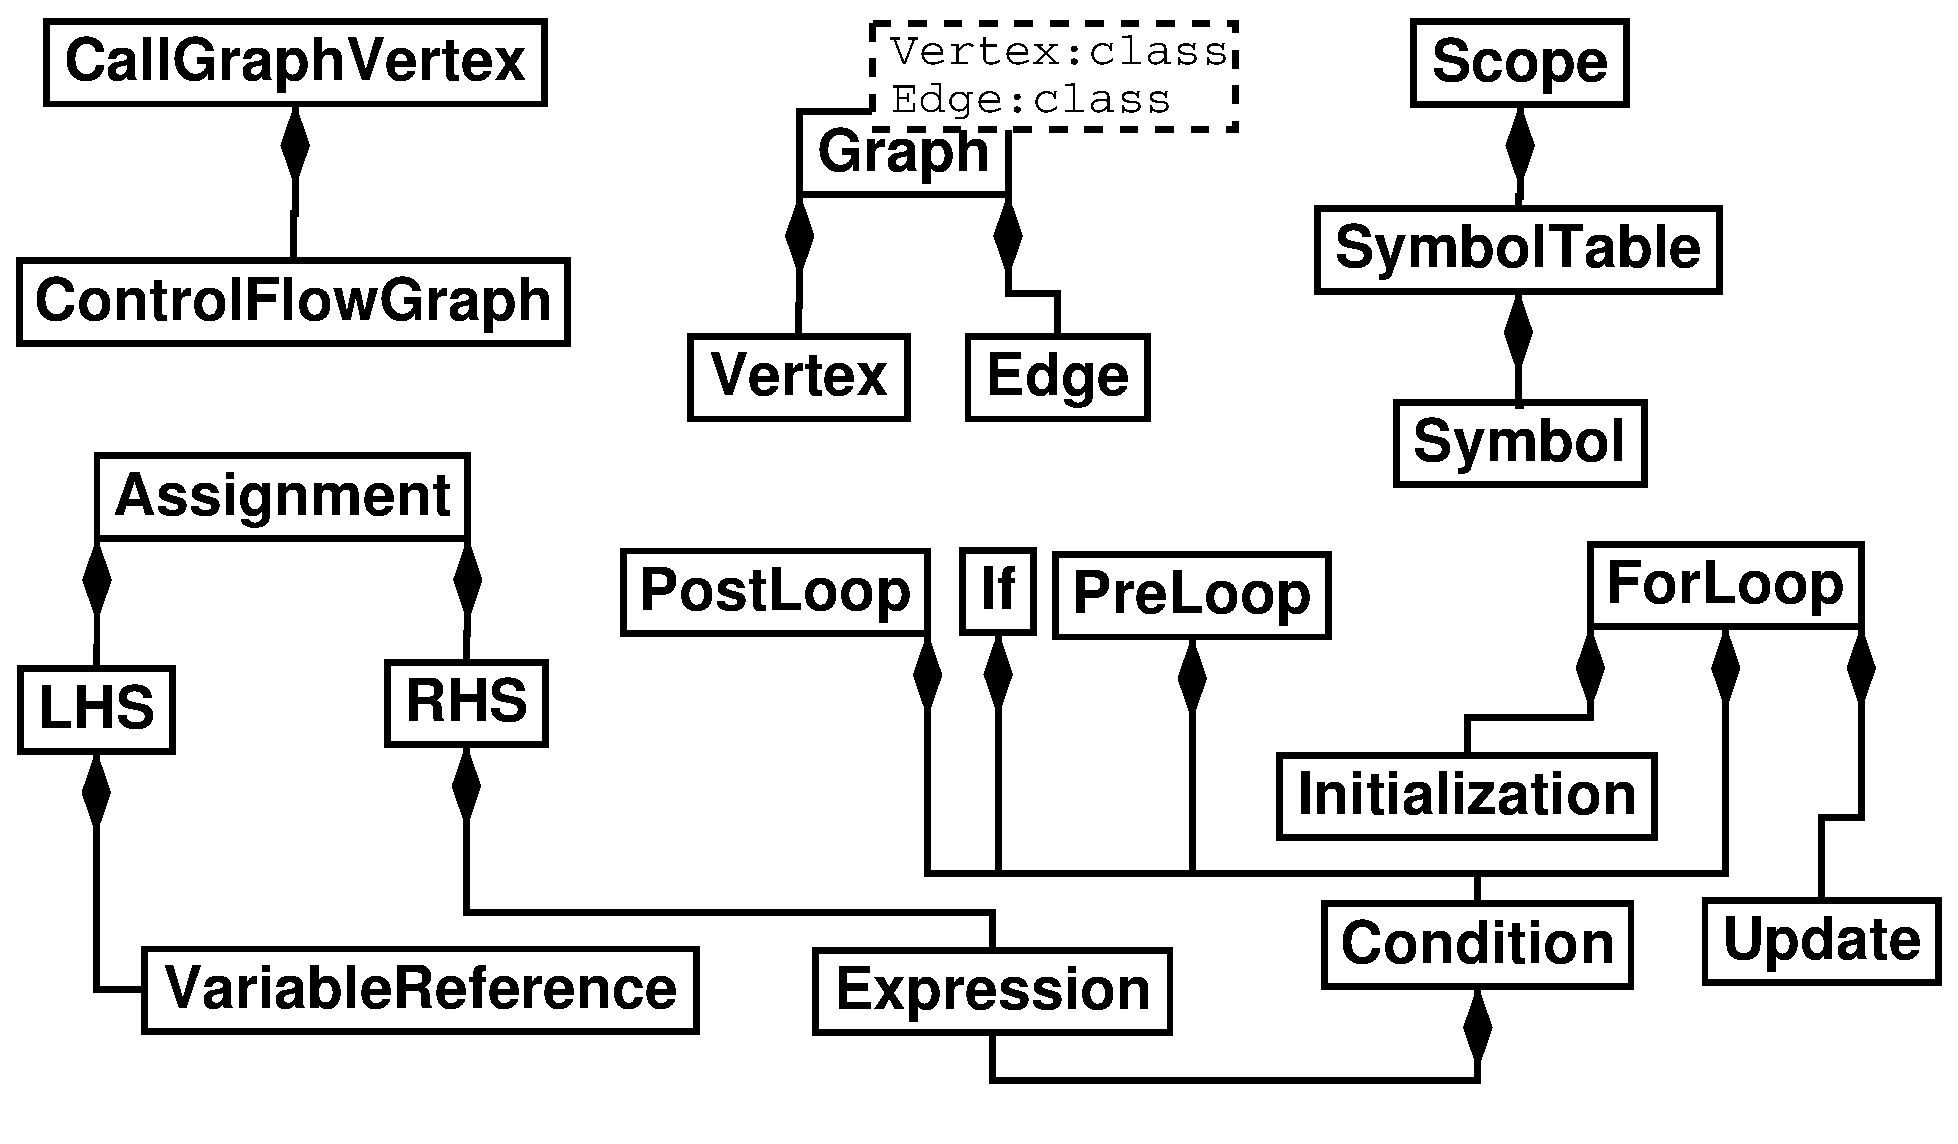
\includegraphics[width=.45\textwidth]{irComp}
  \caption{Simplified class composition in \xaifBooster} \label{fig:irc}
\end{figure}
A doxygen generated documentation of the entire data structure 
can be found on the \OpenAD\ website \cite{openadWeb}.
The class hierarchy is organized top down with 
a single \code{CallGraph} instance as the top element. 
The top down structure is also imposed on the ownership of dynamically 
allocated elements. 
Whereever possible, the class interfaces encapsulate dynamic 
allocation of members.  
Only in cases of containment of polymorphic elements is explicit dynamic allocation 
ouside of the owning class' members appropriate. 
In these cases the container class interface naming and documentation 
indicates the assumption of ownership of 
the dynamically allocated elements being supplied to the container class. 
An example is the graph class \code{Expression} accepting vertex instances that can be 
\code{Constant}, \code{Intrinsic} , etc.

The transformation algorithms are modularized to enable reuse in different 
contexts. 
\begin{figure}
  \centering 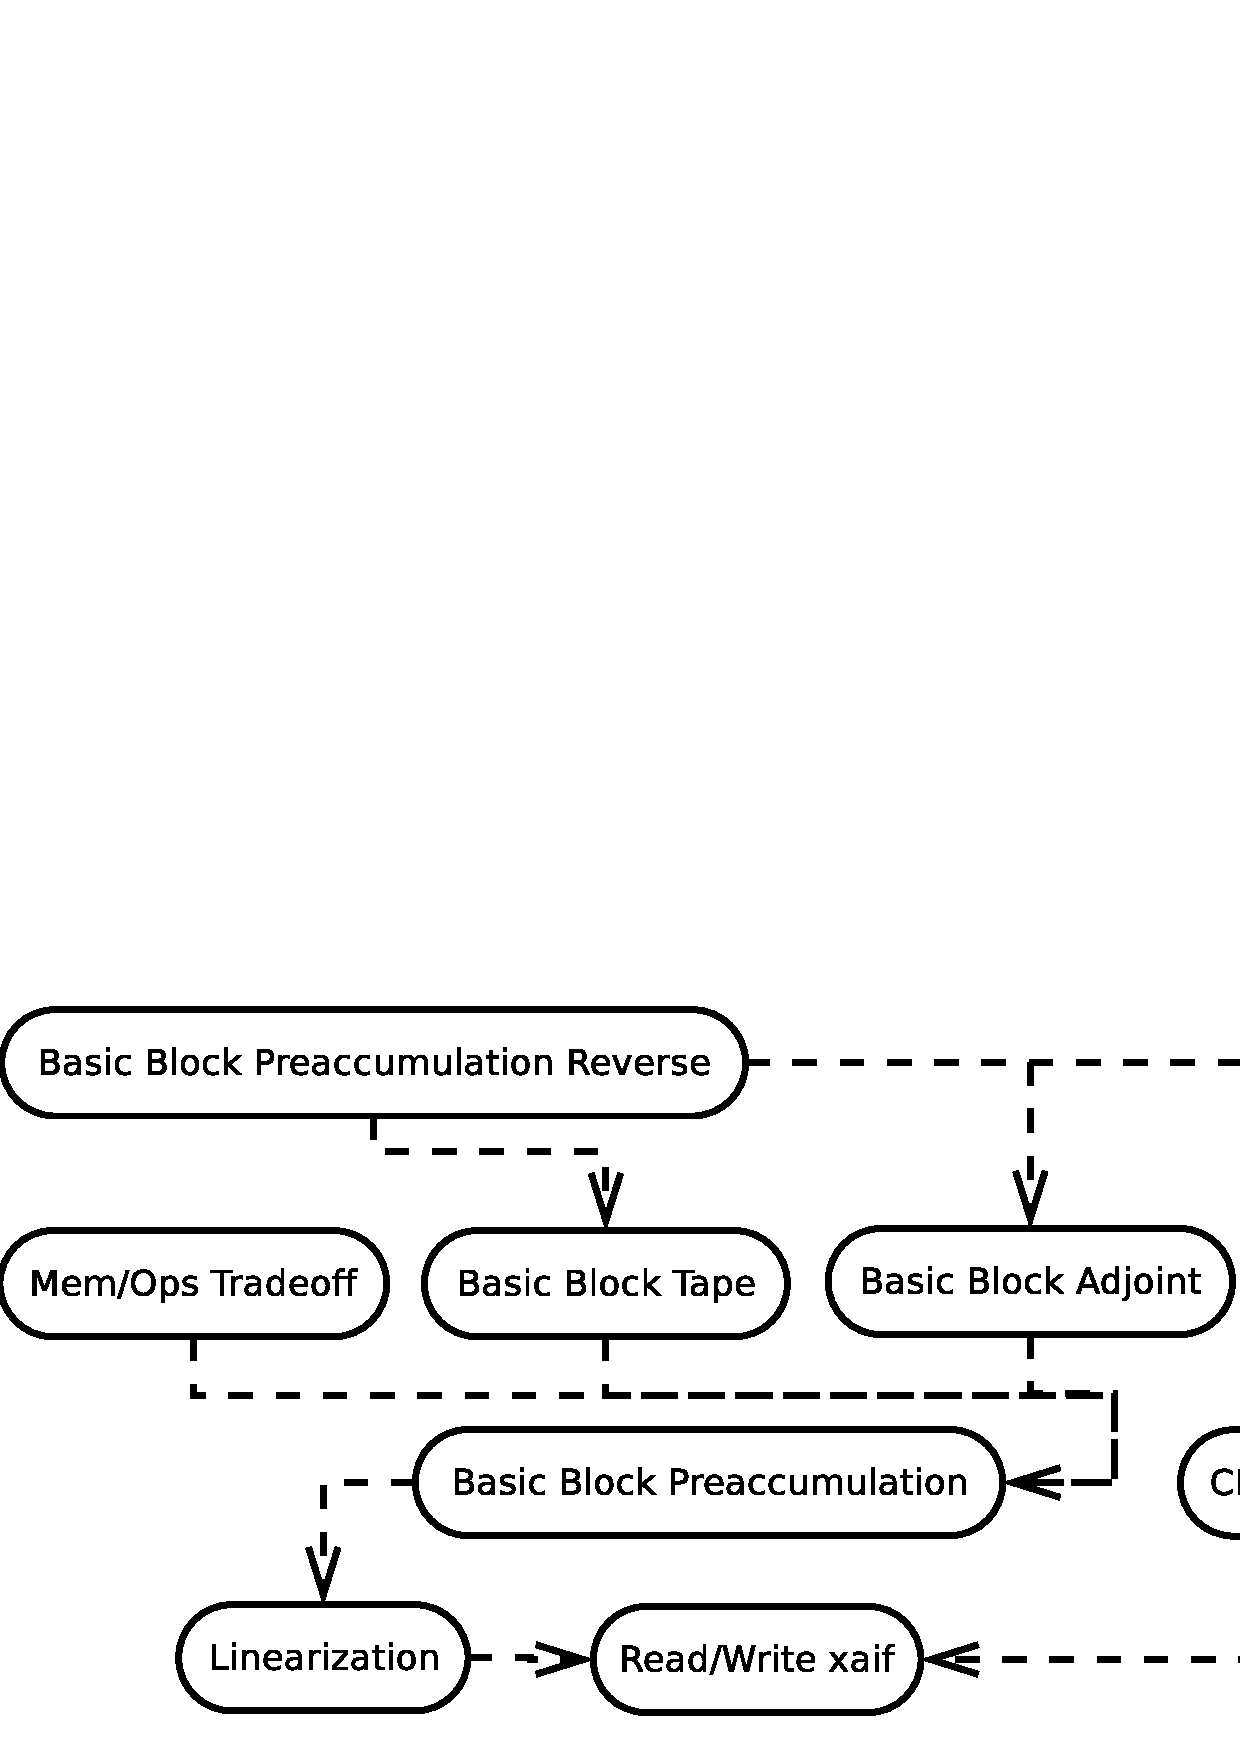
\includegraphics[width=.45\textwidth]{allAlgs}
  \caption{\xaifBooster\ algorithms} \label{fig:allAlgs}
\end{figure}
\reffig{fig:allAlgs} shows some implemented algorithms with dependencies.
To avoid conflicts the transformation algorithms the data structure representing the input code  
is never directly modified. 
Instead, any data representing modifications or augmentations of the 
original representation element in a class \code{<name>}
are held in algorithm specific instances of class \code{<name>Alg}.
The association is done via mutual references accessible 
through \code{get<name>AlgBase()} and \code{getContaining<name>()} respectively.
The instantiation of the algorithm specific classes follows 
the factory design pattern. The factory instances in turn are controlled 
by a transformation algorithm specific \code{AlgFactoryManager} classes. 
Further details can be found in \cite{sea2003}, howeverer, the code 
code for this mechanism is fairly self-explanatory.  

In the following sections we want to concentrate on the transformation 
the algorithms execute while deferring to the generated code 
documentation for most technical details.

Each algorithm has a driver \code{t.pp} (compiled into a binary \code{t}) 
found in \code{algorithms/<the\_algorithm\_name>/test/} 
that encapsulates the algorithm 
in a stand-alone binary which provides the functionality described 
in the following 
sections. For details on the invocation and command line options refer to 
\refsec{ssec:manualPipeline}.

% -----------------------------------------------------------------------------------------
\paragraph{Reading and Writing \xaif}\label{ssssec:readWriteXaif}
Reading and Writing the \xaif\ is part of basic infrastructure
found in the sources in \code{system/}.
Parsing is done through the Xerces C++ XML parser \cite{xercesWeb}
such that the XML element handler implementations, see \code{system/src/XAIFBaseParserHandlers.cpp},
build the \xaifBooster\ data 
structure from the top down. 
As an additional consistency check all components that read \xaif\ data 
have the validation according to the schema enabled. Beyond the schema 
validation these components perform valdity checks. Therefore, 
manual modifications of \xaif\ data , while possible, should 
be done judiciously. 

The unparsing of the transformed data structure into \xaif\ is performed 
through a series of that traverses the data structure and the 
respective algorithm specific data. 
For information of the files containg the \xaif\ representation refer to 
\refsec{ssec:manualPipeline}.

Aside from the parsing of the actual input \xaif\ there is also the so called 
{\em 
  catalogue of inlinable intrinsics
} 
supplied as an XML following a specialized schema in \xaif, see  
\refsec{sssec:linearization} and \refsec{sssec:wtxxtw}.
There is also a driver at this level found in \code{system/test/t.cpp} used 
to verify reading and writing functionality. It can be used to establish 
that the tool pipeline preserves the semantics of the original program when 
no transformation is involved. 

% -----------------------------------------------------------------------------------------
\paragraph{Linearization}\label{sssec:linearization}

\refsec{sec:ADIntro} explained the computation of 
the local partial derivatives $c_{ji}$ that can be thought of as edge labels 
in the computational graph $G$. 
Per canonicalization (see \refsec{sssec:Canonicalization}) 
all elemental $\phi$ 
occur only in the right-hand side of an assignment. 
For each $\phi$ we look up the definition of the respective partials in 
the intrinsics catalogue. 
{\color{red} [ not sure  how much detail is necessary ] } 
The partials are defined in terms of positional arguments, see 
\reffig{fig:divExample}. 
\begin{figure}
  \centering 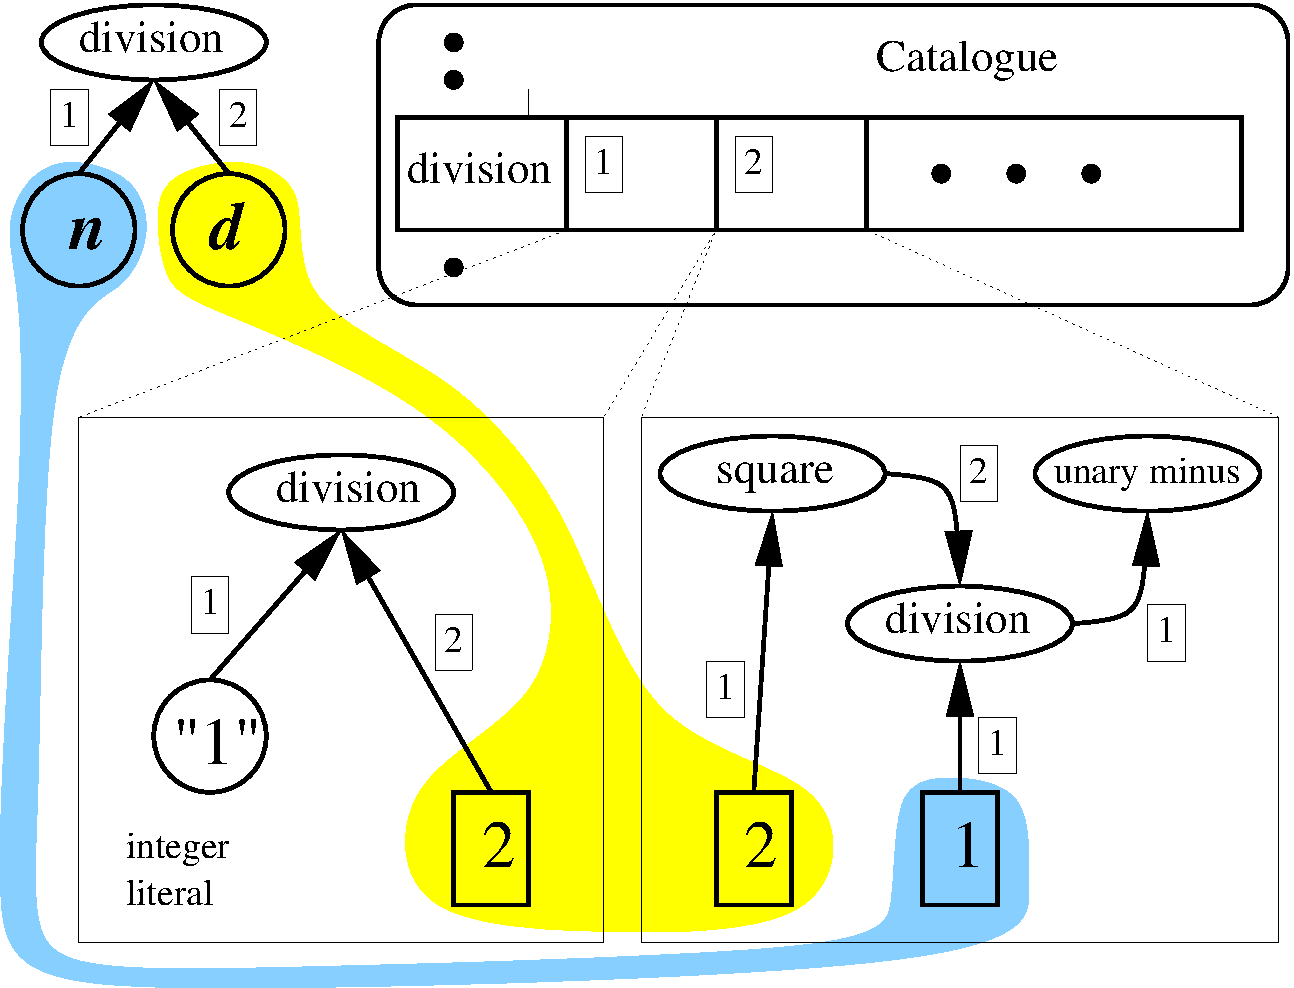
\includegraphics[width=5cm]{divIntrinsic}
  \caption{Partial expressions for the division operator} \label{fig:divExample}
\end{figure}

Because of this, 
the right-hand-side expression may have to be split up into 
subexpressions to assign intermediate values to ancillary variables 
that can be referenced in the partial computation, for an example see 
the code shown in \reffig{fig:toyAndPartials}.  
In cases of the left-hand-side variable occuring on the right-hand-side 
(or being may-aliased to a right-hand-side variable, 
see \refsec{sssec:openanalysis}) we also require an extra assignment to 
delay the (potiential) overwrite until after the partials depending on 
the original variable value have been computed.
The result of the Linearization is a representation for 
code containing the potentially split 
assignments along with assignments for each non-zero edge label $c_{ji}$.
These representations are contained in the \code{xaifBoosterLinearization::AssignmentAlg} instances associated with each assignment in the \xaif.
The generated code after unparsing to Fortran 
is compilable but does by itself not compute useful 
derivative information at the lavel for the target function $\bmf$. The 
transformation driver is 
used to verify the results of the linearization transformation.

% -----------------------------------------------------------------------------------------
\paragraph{Basic Block Preaccumulation}\label{sssec:BBPreacc}

This transformation generates a code representation that can be used 
to compute derivatives in forward mode. It builds upon the Linearization
done in \refsec{sssec:linearization}. 
The first step constructs the 
computational graphs $G$ 
for contiguous 
assignment sequences in a given \basicblock. To ensure semantic 
correctness of the graph being constructed in the presence of 
aliasing it relies on alias analysis and define-use/use-define chains 
supplied by \OpenAnalysis, see \refsec{ssec:openanalysis}.
The algorithm itself is described in detail in \cite{Utk04FBB}.
Because the analysis results supplied by \OpenAnalysis\ are always 
conservatively correct it may not be possible to flatten all 
assignmments into a single computational graph. In such cases 
a sequence of graphs is created. Likewise, the occurence 
of a subroutine call leads to a split in the graph construction. 
In the context of \refsec{sec:ADIntro} one may think of the sets of 
assignments forming each of these graphs as a separate \basicblock. 
The driver for the algorithm allows to disable 
the graph construction across assignments and restrict it to 
single right-hand sides by adding the \code{-S} command 
line flag. 

Based on the constructed $G$ an elimination sequence has to be determined.
To allow a choice for the computation of the elimination sequence 
the code uses the interface coded in \code{algorithms/CrossCountryInterface/}
and by default calls the \angel\ library \cite{angelWeb}.
\angel\ determines an elimination sequence and returns it as 
fused multiply add expressions in terms of the edge references.
There are several heuristics implemented within \angel\ that control 
the selection of elimination steps and thereby the preccumulation code 
that is generated.  The algorithm code calls a default set of heuristics. 
However, all heuristics use the \code{CrossCountryInterface} and therefore 
different heuristics can be selected with minimal changes in algorithm code.   

The second step in this transformation is the generation of 
preaccumulation code. 
First it  turns the abstract expression graphs returned by \angel\ 
into assignments and resolves the edge references into 
the  labels $c_{ji}$. The resulting code resembles what 
we show in  \reffig{fig:toyAccumulation}. 
Then it generates the code that eventually performs the \saxpy\ 
operations shown in \refeqn{eqn:bbfm}. 
Considering the input and output variables $\bmx_j$ and $\bmy_j$ of a \basicblock\ the code generation 
also ensures proper propagation of $\dot{x_i^j}$ of variables $ x_I^j \in  \bmx_j \cap \bmy_j$ 
by saving the $\dot{x_i^j}$ in temporaries. The example in \reffig{fig:toyPreacc} illustrates this case. 
The detection of the intersection elements relies on the alias analysis provided by 
\OpenAnalysis.
To reduce overhead 
the generated \saxpy\ operations we generate \saxpy\ calls following the 
interface specified in \code{algorithms/DerivativePropagator/} for the following four cases:  
$\dot{y} = \frac{\partial y }{\partial x }\cdot \dot{x}$, 
$\dot{y} = \frac{\partial y }{\partial x }\cdot \dot{x} + \dot{y}$, 
$\dot{y} = \dot{x}$, and 
$\dot{y} = 0$.	
The generated code is executable and represents an overall forward mode 
according to \refeqn{eqn:bbfm} with \basicblock\-local preaccumulation in 
cross-country fashion. 

% -----------------------------------------------------------------------------------------
\paragraph{Memory/Operations Tradeoff}\label{sssec:MMTradeOff}

This algorithm can be seen as an alternative to the \angel\ library. 
Like \angel\ it uses the \code{CrossCountryInterface}. In its implementation 
it replaces the call to \angel\ with one to its own internal routines that
determine an elimination sequence according to a selectable set of heuristics. 
In difference to the \angel\ heuristics  they 
aim for a tradeoff between the number of operations required to complete an elimantion 
sequence on the one hand and the temporal locality of the $c_{ji}$ in memory on the other hand. 
The rationale for these heuristics is the observation that in many modern 
computer architectures the performance is memory bound, i.e. a few additional 
operations can easily be absorbed if we keep all the necessary data in cache. 
All heuristics take as an input a set $\Theta \neq \emptyset $ of target elements, that is 
a set of vertices or edges from $G$, or faces from $\cal G$. 
The heuristic selects a nonempty subset $\Theta'\subseteq \Theta $ from this set. 
In order to determine a single elimination target a sequence of heuristics may be applied 
that successively shrink the target set concluding with a tie breaker such as 
selecting the next target that would be eliminated in forward or reverse mode. 
\reftab{tab:memOpsHeur} describes the selection criterion of a heuristics with 
respect to an elimination technique.  If the selection criterion is not met 
by any target in $\Theta$, then $\Theta'=\Theta$. 
\begin{table}[htb]
  \begin{tabular}{|l|c|c|c|}\hline
    & \code{VERTEX} & \code{EDGE} & \code{FACE} 
    \\\hline %---------------------------------------
    \code{SIBLING} 
    &
    \begin{minipage}{.4\linewidth}
      \footnotesize
      select vertices that share at least one predecessor
      and sucessor with the most recently eliminated vertex.
    \end{minipage}
    & N/A & N/A
    \\\hline %---------------------------------------
    \code{SIBLING2} 
    &
    \begin{minipage}{.4\linewidth}
      \footnotesize
      select vertices with the maximal product of 
      the number of predecessors and the number of 
      successors shared with the most recently eliminated vertex
    \end{minipage}
    &
    \begin{minipage}{.2\linewidth}
      \footnotesize
      select edges with the same source / target and the 
      maximal number of successors / predecessors shared with the 
      successors / predecessors of 
      the most recently front / back eliminated edge
    \end{minipage}
    & N/A 
    \\\hline  %---------------------------------------
    \code{SUCCPRED} 
    &
    \begin{minipage}{.4\linewidth}
      \footnotesize
      select vertices  that were either predecessors or sucessors of
      the most recently eliminated vertex
    \end{minipage}
    & N/A & N/A 
    \\\hline %---------------------------------------
    \code{ABSORB} 
    & N/A & N /A &
    \begin{minipage}{.2\linewidth}
      select faces that are absorbed
    \end{minipage}
    \\\hline %---------------------------------------
    \code{MARKOWITZ} 
    &
    \begin{minipage}{.4\linewidth}
      \footnotesize
      select vertices with  the lowest Markowitz degree
    \end{minipage}
    &
    \begin{minipage}{.2\linewidth}
      \footnotesize
      select edges with the lowest Markowitz degree
    \end{minipage}
    &
    N/A
    \\\hline %---------------------------------------
    \code{FORWARD} 
    &\multicolumn{3}{c|}{
      select the target next in forward mode
    }
    \\\hline %---------------------------------------
    \code{REVERSE} 
    &\multicolumn{3}{c|}{
      select the target next in reverse mode
    }
    \\\hline %---------------------------------------
  \end{tabular}
  \caption{Heuristics selection criteria}\label{tab:memOpsHeur}
\end{table}
The driver allows a sequence of heuristics to be seletec via string supplied as 
an argument to the commandline swith \code{-H}. The string needs to contain 
the target selection, one of \code{Vertex}, \code{EDGE}, or \code{FACE} followed by 
a sequence of heuristics that should include at least on of the tie breakers \code{FORWARD} or 
\code{REVERSE}. 
Obviously the data locality criteria still are rather simplistic but 
the code is easily extensible for more elaborate strategies. 

The generated code is executable and represents an overall forward mode 
according to \refeqn{eqn:bbfm} with \basicblock\-local preaccumulation in 
cross-country fashion. 

% -----------------------------------------------------------------------------------------
\paragraph{Using the ANGEL Library}\label{sssec:angel}
{\color{red} [ JU: This was a placeholder to talk about the \angel\ lib 
  but I think I will remove this unless somebody stronly objects]}
% -----------------------------------------------------------------------------------------
\paragraph{CFG Reversal}\label{sssec:cfgRevAlg}

\refsec{ssec:cfReversal} explains the principal approach to the reversal 
of the CFG. The CFG reversal as implemented in this transformation is 
by itself not useful othern than for checking the correctness without 
interference from other transformations. It is a major building block for 
the  
adjoint code generater described in \refsec{sssec:BBRev}. 
The \Loop\ counters and \branch\ identifiers are stored the same 
stack datastructure that is used for the {\em tape} (introduced in 
\refsec{ssec:cfReversal} and also used in \refsec{sssec:bbTA}.  
The reversal of loops and branches as detailed in \cite{NULF04CFR} assumes 
CFGs to be well-structured, that is, essentially to be free of arbitrary jump instructions 
such as \code{GOTO} or \code{CONTINUE}. 
It is of course possible to reverse such graphs, for instance by enumerating
all {\basicblock}s, recording the execution sequence and invoking them according 
to their recorded identifier in  large  \code {SWITCH} statement in reverse order.
Such a reversal is obviously less efficient than a code that, by employing proper 
control flow constructs, aids compiler optimization. 
For the same reason well tuned codes implementing the target function $\bmf$ will 
avoid arbitrary jumps and therefore we have not seen sufficient demand to implement 
a CFG reversal for arbitrary jumps. 

The reversal of  \Loop\ constructs such as \code{do i=1,10} replaces 
the loop variable \code{i} with a generated variable name, say \code{t} and we 
loop up to  the stored execution count which we will call  \code{c} here. 
Then the reversed \Loop\ is \code{do t=1,c}. Quite often the loop body contains 
array derefences such as \code{a(i)} but \code{i} is no longer available in the 
reversed \Loop. We call this kind of \Loop\ reversal {\em anonymous}. 
To access the proper memory location \code{i} will have to be stored along with the 
\Loop\ counters and \branch\ identifiers in the tape stack.
To avoid this overhead the \Loop\ reversal may be declared {\em explicit}
by prepending \code{c\$openad xxx simple loop} to the \Loop\ in question. 
With this directive the original \Loop\ variable will be preserved,  
the reversed \Loop\ in our example constructed as \code{do i=10,1,-1} and 
no index values for the array references in the \Loop\ body are stored. 
In general the decision when an array index needs to be stored is better answered 
with a code analysis similar to TBR analysis \cite{HNP02}. 
Currently we do not have such  analysis available and instead 
as a compromise define the {\em simple}
\Loop\ which can reversed explicitly as follows. 
\begin{itemize}
  \parskip = -2pt
\item \Loop\ variables are not updated within the loop,
\item the \Loop\ condition does not use \code{.ne.},
\item the \Loop\ condition's left-hand side consists only of the \Loop\ variable,
\item the stride in the update expression is fixed,
\item the stride is the right-hand side of the top level \code{+} or \code{-} operator,
\item the loop body contains no index expression with variables that are modified within the loop body.
\end{itemize}
While these conditions can be relaxed in theory, in practice the effort to implement 
the transformation will rise sharply. Therefore they represent a workable compromise 
for the current implementation. 
Because often multidemensional arrays  are accessed with nested loops the 
\Loop\ directive when specified for the outermost loop will assume the validity 
of the above conditions for everything within the \Loop\ body including nested 
\Loop\ and \branch\ constructs. More details on this aspect can be found in 
\cite{scam_jss_se}. 
% -----------------------------------------------------------------------------------------
\paragraph{Writing and Consuming the Tape}\label{sssec:bbTA}

Together with the CFG reversal two more building blocks contribute to the 
generation of adjoint code. 
\refsec{sec:ADIntro} points to the need to store the $\frac{\partial \phi_j}{\partial v_i}$ on the tape. 
The first transformation algorithm handles the writing of the tape.
For the preaccumulation approach we store the nonzero elements of local
Jacobians $\bmJ_j$ instead. The algorithm that tapes these elements reinterprets
the \saxpy\ operations \code{Y=A*X+Y} generated for \refeqn{eqn:bbfm}, see \refsec{sssec:BBPreacc}, 
and instead generates code that stores any nonconstant factors \code{A} in the tape stack. 

The second tranformation algorithm creates the adjoint code for a single \basicblock.
During the subsquent reverse sweep the previously stored factors have to retrieved from the stack and 
the respective adjoint operations for \refeqn{eqn:bbrm} carried out. 
The respective adjoints of the four different categories listed in \refsec{sssec:BBPreacc} are listed in 
\reftab{tab:saxpyAdj}.
\begin{table}
  \begin{tabular}{|l|l|}\hline
    $\dot{y} = \frac{\partial y }{\partial x }\cdot \dot{x}$ &  $\overline{x} = \frac{\partial y }{\partial x }\cdot \overline{y} + \overline{x}$ \\
    $\dot{y} = \frac{\partial y }{\partial x }\cdot \dot{x} + \dot{y}$ & $\overline{x} = \frac{\partial y }{\partial x }\cdot \overline{y} + \overline{x}$ \\
    $\dot{y} = \dot{x}$ 					& $\overline{x} = \overline{y}$ \\
    $\dot{y} = 0$ 						& $\overline{y} = 0$ 
  \end{tabular}
  \caption{\saxpy\ adjoints} \label{tab:saxpyAdj}
\end{table} 



% -----------------------------------------------------------------------------------------
\paragraph{Basic Block Preaccumulation Reverse}\label{sssec:BBRev}



{\color{blue} [ this is old stuff from the abstract]  
  \begin{figure}
    \centering 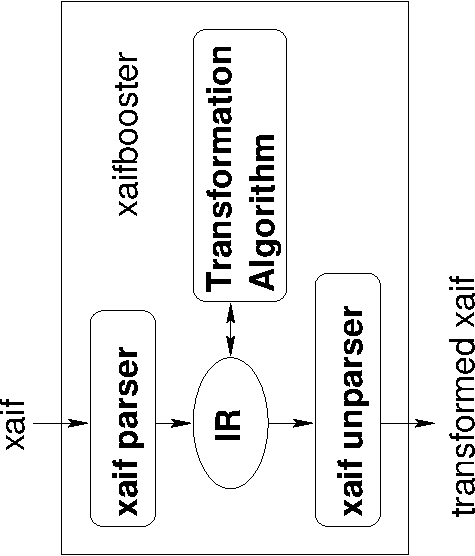
\includegraphics[width=4cm]{principle}
    \caption{\xaifBooster\ parses xaif code into an internal representation (IR).
      It provides an API for transformation algorithms to modify the IR. An unparser
      returns the transformed xaif code.} \label{fig:xaifBooster}
  \end{figure}
  The C++ code \xaifBooster\ is a collection of utilities and routines for the
  (semantic) transformation of programs given in xaif. Its principal architecture 
  is illustrated in \reffig{fig:xaifBooster}. One of the major concerns during
  the development of \xaifBooster\ has been the clean separation of the internal
  representation (an enhanced object image of xaif) from algorithms that operate 
  on this data structure. This goal has been achieved by applying the design 
  patterns \cite{DesignPatterns} factory, visitor, and decorator as described in \cite{UtNa03}.
  The result is an API that gives AD developers the opportunity
  to implement new algorithms in a source transformation environment without
  having to implement full compiler front- and back-ends. Building on
  this API, we have implemented a tangent-linear algorithm that uses statement-
  \cite{SEUpreacc} and basic-block-level preaccumulation of local 
  gradients/Jacobians. Near-optimal face elimination \cite{ElimTechMP} sequences 
  are computed by the software tool 
  ANGEL \cite{AGN03,SAGA} (\code{angellib.sourceforge.net}) and transformed into 
  Jacobian code by
  an \xaifBooster\ algorithm. A simple adjoint version of the code is obtained
  by taping the local Jacobians 
  and by computing the corresponding ``transposed Jacobian-vector" products 
  during an interpretive reverse sweep through the tape. This approach is
  essentially equivalent to split program reversal \cite{Gri00} and allows
  for an easy coupling of tangent-linear and adjoint versions of small to 
  medium-sized codes as described in \cite{NaHe03}. 

  Details of the automatic generation of adjoint code in split mode are presented
  in the full version of the paper. Furthermore, additional information is 
  provided on \xaifBooster\ as a platform for implementing new AD algorithms with 
  the objective to establish an open quasi-standard development infrastructure
  within the AD community.
}


% -----------------------------------------------------------------------------------------
\subsection{\OpenADFortTk\ - the Fortran~90 Front-End}\label{ssec:fortfe}

Every subroutine consists of a {\em control flow graph} (CFG) that 
represents the typical control flow constructs such as \entry, \exit, \Loop, \branch, 
and \basicblock. 
A \basicblock\ consists of a sequence of assignments and subroutine calls. 
In the following we assume some canonicalizations are performed. 
These canonicalizations are implemented in the front end discussed in 
\refsec{sssec:Canonicalization}.
\begin{Can} \label{can:funcToSub}
  All constructs occuring in \basicblock\ that are neither assignments nor subroutine calls (such as function calls, built-in I/O statements) 
  are canonicalized into subroutine calls.
\end{Can}
\begin{Can} \label{can:assignSideEffectFree}
  An assignment effects a single variable on the left-hand side and 
  the right-hand-side expression is side-effect free.
\end{Can}
\begin{Can} \label{can:assignElemental}
  The right-hand-side expression consists only of elemental operations $\phi$ typically 
  defined in a programming language as built-in operators and intrinsics.
\end{Can}
\begin{Can} \label{can:assignFunction}
  User defined functions and calls to these functions in right-hand-side expressions 
  are canonicalized to subroutined calls.
\end{Can}

The main target application of the ACTS project is the MIT general
circulation model (MITgcm) \cite{mars-eta:97b,mars-eta:97a}.
It is mostly implemented in Fortran~77 to permit maintenance of an
efficient and correct adjoint as the code evolves \cite{HHG02}. Future
development will increasingly add Fortran~90 features.  The
\OpenADFortTk\ (OpenAD Fortran Toolkit) 
component covers the
Fortran-specific features of the OpenAD system. Throughout this
paper, we use ``front-end'' as a synonym for \OpenADFortTk.

In spite of the appellation ``front end'', \OpenADFortTk\ subcomponents
operate at several stages of the pipeline in the following order.

\begin{enumerate}	
\item \mfefninety\ is a compiler front-end in the classical sense that parses
  Fortran and generates an intermediate representation (IR)
  in the \whirl\ language

\item The {\em canonicalizer} converts  
  programming constructs into the canonical form required by 
  \refcan{can:funcToSub} - \refcan{can:assignFunction}. 
  This component modifies \whirl\ in core.

\item \whirlToxaif\ is a bridge component that
  \begin{itemize}
  \item drives the various program analyses (see \refsec{ssec:openanalysis}),

  \item filters out program statements that are not in the
    computational core of the language, and 

  \item converts the program analyses and core computational
    statements from \whirl\ into \xaif.
  \end{itemize}

\item \xaifTowhirl\ is bridge component that converts the 
  differentiated program represented in \xaif\ 
  to a \whirl\ representation.

\item \whirlTof\ is the ``unparser'' that converts \whirl\ to
  Fortran.

\item The {\em postprocessor} is the  final part of the transformation that
  performs template expansion as well as inlining substitutions.

\end{enumerate}

In the following we will explain the subcomponents in more detail.
The invocation of the components is explained in
\refsec{ssec:manualPipeline}

% -----------------------------------------------------------------------------------------
\subsubsection{\OpenSixtyFour\ components} \label{sssec:mfef}

The \OpenSixtyFour\ project \cite{open64Web} supplies two elements for
the front end, \mfefninety\ and \whirlTof.

To ensure robustness of the AD tool, we sought industrial strength
programming-language-dependent components.  We chose the Center for
High Performance Software Research's (Rice University) \OpenSixtyFour\
compiler, a multi-platform version of the SGI Pro64/Open64 compiler
suite, originally based on SGI's commercial MIPSPro compiler.
\OpenSixtyFour's Fortran front end, \mfefninety, is a classical
compiler parser that reads Fortran source and converts it to an
intermediate language called \whirl.  A companion tool, \whirlTof,
unparses \whirl\ back to Fortran source code.  The \whirl\
representation, which resembles a typical abstract syntax tree, has
been designed to enable good optimization for high performance
computing in Fortran, C, and C++. See \cite{open64Web} for more
details about the intermediate language.  HiPerSoft's main
contribution to the \OpenSixtyFour\ community has been extending the
infrastructure to support source-to-source transformations; thus, it
has invested significant effort in the \whirlTof\ unparser.

AD tools require certain knowledge that typically is not directly
representable in programming languages such as Fortran.  For example,
an AD tool must know what variables in the code for $\bmf$ are
independent and dependent.  Instead of suppling this information
externally, such as with a configuration file, we introduced a special
OpenAD pragma facility, encoded within Fortran comments, and extended
\OpenSixtyFour\ to generate and unparse OpenAD pragma nodes in \whirl.
Similar to many other special-purpose Fortran pragmas systems such as
OpenMP \cite{OpenMP-website}, in order to specify that a variable
$y$ is dependent, a user could write \code{!\$openad dependent(y)},
where \code{\$openad} is the special prefix that demarcates OpenAD
pragmas.  Unlike most pragma systems, we introduced a generic
\code{!\$openad xxx} pragma\footnote{The mneumonic behind name is that
  as $x$ is the typical variable name, so \code{!\$openad xxx} is the
  `variable' pragma.} that can communicate arbitrary pieces of
text--associated with whole procedures, single statements, or groups
of statements--through the pipeline.  This generic pragma provides a
flexible system for experimentation and eliminates the significant
development costs associated with modifying \OpenSixtyFour.


% -----------------------------------------------------------------------------------------
\subsubsection{Canonicalization}\label{sssec:Canonicalization}

To ensure the language independence of the transformation engine and
streamline its development, the front end converts and simplifies some
programming constructs into \emph{canonical} form.  In addition to the
canonicalizations mentioned in \refsec{sec:ADIntro} language
independence requires the following:

\begin{Can}\label{can:comBlock}
  Common blocks are converted to modules.
\end{Can}
\begin{Can}\label{can:param}
  Non-variable actual parameters are hoisted to temporaries.
\end{Can}
\begin{Can}\label{can:scalar}
  Derived type references are scalarized.
\end{Can}	


{\color{red}
  Canonicalization is 

  [ expand on reason for canonicalization: 
  1) make life easier for whirl2xaif
  2) XAIF's limited concepts (explained below) 
  ] \\

  [ how are canonicalizations implemented: on whirl instead of fortran ] \\

}

All canonicalizations are implemented as part of \whirlToxaif; see 
\refsec{sssec:wtxxtw}.

% -----------------------------------------------------------------------------------------
\subsubsection{\whirlToxaif\ and \xaifTowhirl}\label{sssec:wtxxtw}

\begin{figure}
  \scriptsize
  \verbatimfile{code/daerfj.f90}
  \caption{Example Fortran code}\label{fig:exampleFortranCode}
\end{figure}

\begin{figure}
  \scriptsize
  \verbatimfile{code/daerfj.whirl}
  \caption{Part of whirl for \reffig{fig:exampleFortranCode}}\label{fig:exampleWhirlCode}
\end{figure}

\begin{figure}
  \scriptsize
  \verbatimfile{code/daerfj.xaif}
  \caption{Part of \xaif\ for \reffig{fig:exampleFortranCode}}\label{fig:exampleXaifCode}
\end{figure}


An important part of the pipeline is the translation of \whirl\ into
\xaif\ (\whirlToxaif), feeding it to the transformation engine, and
then backtranslating the differentiated \xaif\ into \whirl\
(\xaifTowhirl).  Two distinguishing features of \xaif\ shape the
contours of \whirlToxaif\ and \xaifTowhirl.  First, because \xaif\
represents only the numerical core of a program, many \whirl\
statements and expressions cannot be translated into \xaif\.  For
instance, in \xaif\ there is no way to represent Fortran IO statements
or expressions involving user-defined types or array slices.  We
therefore introduced special statements and annotations to \xaif\ in
which opaque information can be stored.  These opaque objects, which
refer to the input \whirl, are created by \whirlToxaif\ and deposited
in the special \xaif\ constructs designed for conveying such
information through the differentiation engines.  Given the original
\whirl\ and the differentiated \xaif\ (with the opaque objects
intact), \xaifTowhirl\ generates new \whirl\ representing the
differentiated code.  

The second distinguishing characteristic of \xaif\ is that it
represents programs in a format similar to that used by common
compiler analyses.  For example, a program is a call graph and a
collection of associated symbol tables where nodes in the call graph
are CFGs.  Hence, \whirl\ control flow statements are implicitly
represented by CFG nodes and edges where the former are {\basicblock}s
containing non-control-flow statements.  Moreover, symbol table
entries, statements and variable references in \xaif\ are annotated
with information from data flow analyses such as alias analysis, ud-
and du-chains, and activity analysis.  \whirlToxaif\ uses the
\OpenAnalysis\ package to collect all of this information before
proceeding with the translation into \xaif.  In doing so, it
implements the OA interface to \whirl, invokes the necessary analyses,
and massages the results into a form consistent with \xaif.

\xaifTowhirl\ backtranslates \xaif\ into \whirl\ that includes
postprocessor directives.  It performs no transformations and
therefore has no use any analysis information that might be included
in the source \xaif.  Consequently, its challenges during
backtranslation are to recover explicit statement-based control flow
constructs from the CFG; correctly restore any \whirl\ represented by
opaque objects (which were inserted by \whirlToxaif); and introduce
any necessary postprocessor directives, most important of which
indicate that active variables should be converted to structured types
and that active references should include an approprate value or
derivative selector.

{\color{red} [ how are intrinsics handled ... I refer to the catalogue later  ] }



\subsubsection{Postprocessor}\label{sssec:PostProcessor}
The postprocessor performs various ``cleanup'' operations of the
differentiated code. The two most important tasks are:
\begin{enumerate}
\item template expansion
\item inline substitution
\end{enumerate}

Template expansion is intimately connected with the differentiation
algorithms. Some parts of the code use different recomputation/storage
strategies, as well as different taping patterns. These various
strategies are encoded in Fortran templates, and expanded by the
post processor.

Similarly, some operations introduced by the differentiation process
are coded as function operations. To make these operations work well,
however, they must be substituted inline, replacing the function call.

{\color{red}
  [ Need examples of templates here (or somewhere) ]

  [ Does inlining serve any other purpose besides efficiency?  Yes --
  the inlined routines have strange parameter substitution to support
  the active data-structures.]

  [postprocessor to handle things that are not convenient to do in whirl
  (making xaif2whirl's life easier).]
}



% #########################################################################################
\section{Tool Usage} \label{sec:Usage}
The following contains brief instructions how to obtain and use \OpenADF. 
While the principal approach will remain the same, future development may 
introduce slight changes. The reader is encouraged to refer to the 
up to date instructions on the \OpenADF\ website \cite{openadWeb}.
\subsection{Download and Build}\label{ssec:dab}
\subsection{Automatic Pipeline}
\subsection{Manual Pipeline}\label{ssec:manualPipeline}


% #########################################################################################
\section{Application}\label{sec:application}

The reference application for the first prototype of an \OpenADF\ implementation
is a simplified oceanographic box model for investigating
thermohaline circulation. It relates to the
ocean circulation's role in the variability of the climate system,
on time scales of decades to millennia \cite{tzi-ioa:02}.
Previously, the AD tool TAF \cite{GiKa02} 
had been used to generate the derivative
code in both forward and reverse modes.
See \cite{maro-eta:99} for an applications of
TAF's predecessor TAMC to the MITgcm.

\OpenADF\ has been used to generate tangent-linear and 
adjoint versions of the box model. We established numerical identity between
the Jacobians provided by TAF and \OpenADF.
The successful 
application of \OpenADF\ to the box model code is considered as a feasibility 
proof for the overall approach taken by the ACTS project.  
% -----------------------------------------------------------------------------------------
\subsection{Shallow Water Model}
% -----------------------------------------------------------------------------------------
\subsection{Derya's application}
% #########################################################################################
\section{Conclusion and Future Work}\label{sec:concl}

{\color{red} dynamic memory}

\OpenADF\ is an AD tool development infrastructure. Its well-separated components
allow developers to focus on various aspects of source-to-source 
transformation AD, including parsing and unparsing of different programming
languages, data and control flow analysis, and (semantic) transformation 
algorithms. The intention of \OpenADF\ is to provide the AD community with 
an open, extensible, and easy-to-use platform for research and development
in the field. Its intention is not to render obsolete existing source transformation
tools such as ADIFOR \cite{adiforWeb}, 
the differentiation-enabled NAG Fortran 95 
compiler,\footnote{\code{http://www.nag.co.uk/nagware/research/ad\_overview.asp}} TAF,\footnote{\code{http://www.FastOpt.de}} and TAPENADE.\footnote{\code{http://tapenade.inria.fr:8080/tapenade/index.jsp}} 
Their closer coupling with the language-specific internal representation of 
the program has the potential to make the
exploitation of certain language features easier. \OpenADF\ is supposed to 
complement these tools by providing well-defined APIs to an open internal 
representation that can be used by a large number of AD developers.
Users of AD technology will benefit from the expected wide
variety of combinations of front-ends and algorithms that is made possible
by \OpenADF.

During the remainder of the ACTS project we will focus on the implementation
of robust and efficient data flow algorithms in \OpenAnalysis, including alias, 
define-use and use-define, in-out \cite{Muc97}, 
activity, and to-be-recorded \cite{HNP02} as well as on 
the development of various reverse mode algorithms for parallel MPI codes
combining elements such as preaccumulation and (automatic) checkpointing
\cite{Gri92}. 
A second set of target 
applications in chemical engineering \cite{FTB97} requires combinations of first and 
second derivatives in addition to methods for exploiting structure and sparsity
of the underlying computation. We intend to investigate ways to compute these
combinations efficiently by integrating \OpenADF\ into the relevant 
numerical algorithms.

Ultimately, our aim is to generate correct, efficient, scalable, and easily 
maintainable adjoint code for the MITgcm. The major challenge arises from the
requirement to tackle problems in which derivatives are calculated with respect 
to billions of controls. A combination of the methods outlined above is 
essential to guarantee the successful completion of this highly ambitious
project.

% #########################################################################################
\section*{Appendix}
\begin{table}
  \tiny
  \begin{center}
    \begin{tabular}{ll}
      {\tt Makefile} & the top level {\tt Makefile}\\
      {\tt utils/} & utility classes (debugging, generic traversal, etc.)\\
      {\tt tools/}  & code generator supporting \xaif\ parser \\
      {\tt boostWrapper/}& wrapper classes for the boost graph library \\
      {\tt system/} & all basic data structures, \xaif\ (un)parsing, \refsec{ssssec:readWriteXaif}\\
      {\tt algorithms/}& see the subdirectories below\\
      \quad{\tt CodeReplacement} & support library for subroutine templates\\
      \quad{\tt CrossCountryInterface} & support library for elimination strategies, \refsec{sssec:BBPreacc}\\
      \quad{\tt DerivativePropagator} & support library for Jacobian vector products\\
      \quad{\tt InlinableXMLRepresentation } & support library for inlinable subroutine calls\\ 
      \quad{\tt Linearization} & Linearization transformation, \refsec{sssec:linearization}\\ 
      \quad{\tt BasicBlockPreaccumulation} & elimination with \angel\ and \\
      & preaccumulation at the \basicblock\ level, \refsec{sssec:BBPreacc}\\
      \quad{\tt  MemOpsTradeoffPreaccumulation} & as above but with different heuristics than \angel\\
      \quad{\tt ControlFlowReversal} & control flow graph reversal\\
      \quad{\tt BasicBlockPreaccumulationReverse } & adjoint code\\
      \quad{\tt BasicBlockPreaccumulationTape } & taping code supporting adjoint\\
      \quad{\tt BasicBlockPreaccumulationTapeAdjoint } & reverse sweep portion supporting adjoint\\
    \end{tabular}
  \end{center}
  \caption{Directory structure in \xaifBooster}\label{tab:dirStruct}
\end{table}


% \bibliographystyle{acmtrans}
\bibliographystyle{plain}
\bibliography{openad}


% \begin{received}
%   Received May 2005;
% \end{received}

\end{document}
